
%: ----------------------- introduction file header -----------------------


% the code below specifies where the figures are stored
\ifpdf
    \graphicspath{{introduction/figures/PNG/}{introduction/figures/PDF/}{introduction/figures/}}
\else
    \graphicspath{{introduction/figures/EPS/}{introduction/figures/}}
\fi

% ----------------------------------------------------------------------
%: ----------------------- introduction content ----------------------- 
% ----------------------------------------------------------------------
\chapter{First Things First}
\section{Cosmic Context}\label{sec:CosmicContext}

The subject of this thesis is the ``Epoch of Reionization", also known as ``hydrogen reionization" or ``reionization" or simply the ``EoR". Let us start with a brief description of what this process is, how it relates to the evolution of the Universe as a whole, and what the open problems are regarding reionization that we are trying to solve. 


The problem of reionization arises when trying to reconcile observations of the early Universe with those of the present-day Universe. Namely, Big Bang nucleosynthesis and observations of the Cosmic Microwave Background (CMB, discussed in \S \ref{sec:CMB})\gloss{CMB}{Cosmic Microwave Background. This is the earliest available snapshot of the Universe and is composed of light which has travelled from the surface of last scattering to today, largely unimpeded.} demonstrate that, when the Universe was $\sim$380,000 years old, neutral hydrogen and helium constituted the vast majority of the baryonic matter. However, observations of nearby quasars (specifically, the \lya\ forest, discussed in \S \ref{sec:LyaForest}) demonstrate that the gas between the galaxies, dubbed the intergalactic medium (IGM)\gloss{IGM}{Intergalactic medium. This refers to the gas between galaxies, which constitutes most of the baryonic matter in the Universe.}, today is almost entirely ionized.\footnote{In \S \ref{sec:LyaForest}, we discuss how the lack of \lya\ absorption in quasar spectra is suggestive of a highly-ionized IGM. However, when this was first observed in 1965 (\citealt{1965ApJ...142.1633G}), it was not obvious that this was indicative of an \textit{ionized} IGM rather than a scenario where galaxy formation was so efficient as to remove almost all of the gas from the IGM. See \cite{meiksin2009physics} for a nice review of the physics of the IGM.} Therefore, it must be the case that some very energetic process occurred in the intervening $\sim$13 billion years which stripped the electrons from almost all of the atoms in the IGM. We refer to this process as the Epoch of Reionization.


Technically, several ionizations have to take place: ionizing hydrogen, singly ionizing helium, and doubly ionizing helium with the required energies per ionization being 13.6 eV, 24.6 eV, and 54.4 eV, respectively. Since the first two processes require roughly the same energy, they are thought to occur concurrently. However, the complete ionization of helium requires four times as much energy as for hydrogen and likely occurs significantly later and as a result of a different process (see, e.g., \S 6.3.2 of \citealt{barkana2001beginning}). For this thesis, we focus exclusively on hydrogen ionization and the single ionization of helium and treat the term ``reionization" as being synonymous with this. 


\begin{figure}[h]
  \centering
  \includegraphics[width=14cm]{BellUniverse.eps}
  \caption{Milestones in the evolution of the Universe from the Big Bang to today.(Photo from NASA WMAP science team)}
  \label{fig:NASAWMAP}
\end{figure}


To help understand where reionization fits into the evolution of the Universe as a whole, we can refer to Figure \ref{fig:NASAWMAP}, which shows the qualitative evolution of the Universe starting with the inflation and the CMB on the far left and ending with the present-day Universe on the right and spanning $\sim$13.8 billion years. One of the exciting aspects of reionization is that so little about it is known for sure. However, a reasonable round-number placement of reionization in this figure would be that it was an extended process that occurred somewhere between $\sim$500 million years after the Big Bang and 1 billion years after the Big Bang, likely coinciding with the formation of the first galaxies. 


The manner in which reionization progressed is also not known for sure and depends on the specifics of what energetic process is at its root. For example, if ``softer" sources, emitting ionizing radiation in the UV but not X-ray, drove reionization, then these photons will see a relatively high photoionization cross section and will not travel far before ionizing hydrogen in their path. Under this scenario, the state of the Universe during reionization would likely resemble a two-phase medium with ionized regions surrounding the ionizing sources and sharp boundaries between the ionized regions and the neutral IGM. Eventually, as the ionized regions grew, they would overlap until the entire IGM was ionized. This is the expected course for reionization in the event that it is driven by the first galaxies.	


If reionization is driven by sources with a ``harder" spectrum, emitting ionizing radiation strongly in X-ray, then the photoionization cross section of these photons will be relatively low. This is because, for photons with $E_{\gamma} \gg 13.6e\text{V}$, the cross section falls off as $\sigma \sim 1/\nu^3$. Because of this, ionizing radiation from these sources will travel \textit{farther} on average before ionizing a hydrogen atom. This will result in transitions between fully-ionized regions and fully-neutral regions being more gradual. This is the expected scenario in the case where reionization is driven by X-ray binaries or quasars. 


Additionally, \cite{McQuinn2007} investigate how the morphology of ionized regions depends on how massive the ionizing sources are. In Figure \ref{fig:McQuinnMorph}, \cite{McQuinn2007} show several reionization simulation outputs. Each panel shows the ionization field for a snapshot of a simulation. Black regions are neutral and white regions are ionized. In each row, the fraction of hydrogen atoms in the IGM that are neutral (dubbed the neutral fraction, denoted $\axhi$) is fixed and decreases for lower rows. Each column corresponds to a different mass distribution for the ionizing sources, with the masses essentially increasing as you move rightward (and assuming galaxies ionize the Universe). As such, the rightmost column demonstrates a plausible reionization scenario when very rare and massive sources dominate the ionizing photon budget. We can see this results in larger ionized regions for a fixed neutral fraction and sharper boundaries between the neutral and ionized regions. On the other hand, the left-hand columns correspond to a relatively larger contribution to the ionizing photon budget from less-massive sources. The result is a more homogeneous ionization with the ionized regions being smaller on average. Despite the uncertainties in the nature of reionization, Figure \ref{fig:McQuinnMorph} gives a qualitative picture of how reionization likely progressed: with ionized bubbles forming around sources, growing, and eventually overlapping until the effectively occupy the entire IGM. 


\begin{figure}[h]
  \centering
  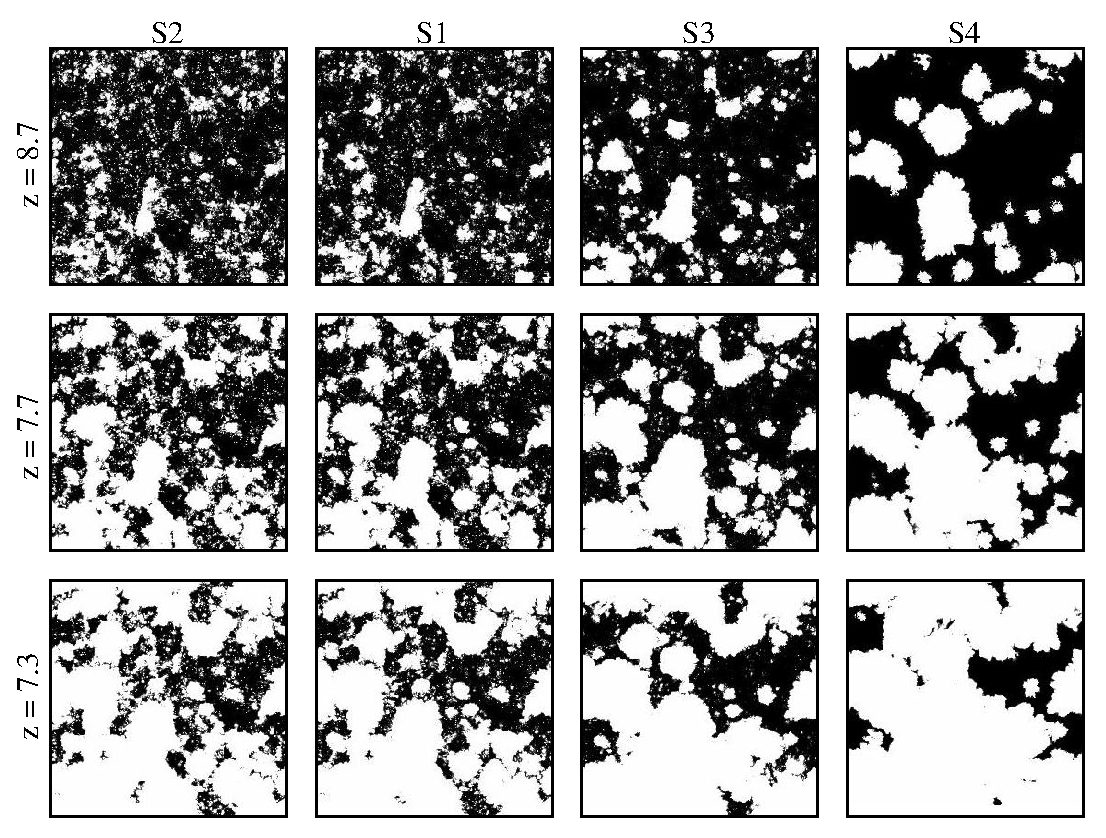
\includegraphics[width=14cm]{McQuinnHIITopology.eps}
  \caption{Simulation outputs from \cite{McQuinn2007} showing four different reionization models. Each row is at fixed $\axhi$ with $\axhi = 0.8$ (top), 0.5 (middle), 0.3 (bottom). The luminosities of the ionizing sources are related to their mass by $\dot{N} \propto m^{1/3}$ (left), $\dot{N} \propto m$ (left-middle), $\dot{N}\propto m^{5/3}$ (right-middle), and $\dot{N} \propto m$ but with a larger minimum mass (right). }
  \label{fig:McQuinnMorph}
\end{figure}


With this qualitative picture in mind, it may be worth emphasizing why astrophysicists and cosmologists care about reionization in the first place. First, the Epoch of Reionization is a significant missing piece in the story of the evolution of the Universe and represents a period in the history of the Universe where we have very few direct observations. Work towards understanding reionization is in line with the overarching goal of pushing observations further and further back in time. Second, the Epoch of Reionization marks the time when radiation from luminous sources became the dominant influence on the IGM and understanding the source of this radiation is interesting in its own right. Understanding the evolution in the properties and number of these bright sources is essential for complete cosmological models. Additionally, while the best guess for the source of the ionizing radiation is dwarf galaxies, it is possible that reionization studies will reveal more exotic and unexpected scenarios, such as annihilating dark matter playing a significant role. Third, the temperature and ionization state of the gas in the Universe plays a regulatory role in galaxy formation: hot and ionized gas will take longer to cool and collapse than cold neutral gas. Since reionization significantly affects both the temperature and ionization state of the gas, understanding reionization will be essential for understanding subsequent galaxy formation. 


Toward these goals, astrophysicists and cosmologists are striving for a thorough understanding of the timing and nature of reionization. When did it happen? How long did it take? What were the ionizing sources? What were the properties of the ionized regions and how did they evolve? These are the questions we should keep in mind throughout the rest of this thesis.


\section{The Shoulders of Giants} 

Before we continue, it is first worth appreciating the difficulty of what we are trying to do. Essentially, we care about measuring the properties of the intergalactic gas -- not stars or galaxies -- when the Universe was only $\lesssim$1 billion years old, a seemingly impossible task. Fortunately, we are given the invaluable gift that light travels at a finite speed and, as such, if we look at distant objects, we see them as they were in the past. Therefore, if we look at the at the gas between galaxies $\sim$13 billion light years away from us, we will see it as it was roughly 13 billion years ago, when the Universe was only 1 billion years old. This means that, in principle, this information of how the young IGM evolved is directly available to us. However, even taking this into account, the intergalactic gas we care about is not bright and it is located extremely far away, so how are we supposed to observe it? An inspiring aspect of studying the Epoch of Reionization is that, when confronted with such a seemingly impossible task, experts in the field have developed many different creative approaches toward constraining the properties of the young IGM. It is this impressive body of work that we aim to build upon. We discuss a selection of the existing and future methods for constraining the EoR in this chapter in order to provide some context and motivation for our work. 

\subsection{The \lya\ Forest}\label{sec:LyaForest}
Arguably the most powerful tool for constraining the high-redshift IGM to date has been the \lya\ forest\nomenclature[Zp]{\lya\ Forest}{This describes the pattern of absorption lines seen blueward of the rest-frame \lya\ line, typically in quasar spectra. These absorption lines can be due to significantly neutral gas in the diffuse IGM or due to dense ionized gas.}. This refers to the pattern of absorption lines seen in the spectra of distant bright objects due to intervening hydrogen, as we will discuss. The \lya\ forest results, in part, from another invaluable gift to the field of cosmology: the redshifting of light with the expansion of the Universe. As the Universe expands, space itself expands and with it the wavelengths of photons travelling through it expand as well. If we know the expansion history of the Universe, and know the intrinsic color of a luminous object, then we can use its \textit{observed} color to determine our distance to the object. Because of this relationship, distances to objects are often measured as a redshift\nomenclature[Zp]{Redshift}{A quantity commonly used to refer to cosmic periods of time or distances. The redshift of an object or location in space is defined as the fractional increase in wavelength that a photon undergoes due to the expansion of the Universe while travelling from the object or location to us.}, defined as the fractional increase in wavelength that a photon experiences when travelling from a given distance to us, denoted by $z$ and defined according to the expression: 

\begin{align}
\lambda_{\text{observed}} &= \lambda_{\text{emitted}}(1+z_{\text{emitter}}). 
\end{align}

The \lya\ forest is seen in the spectrum of extremely bright background objects, usually quasars \gloss{Quasar}{It's bright, OK?} or gamma-ray bursts (GRBs)\nomenclature[Zp]{GRB}{Gamma-Ray Burst. They are also really bright, OK?}, after their light has been processed by the intervening gas. Since the intervening gas is primarily composed of hydrogen and since this hydrogen is generally in the ground state, any intervening neutral patches will absorb light from the background object at the Lyman-series\gloss{Lyman Series}{The series of transitions in an atom where an electron is transitioning to or from the ground state.}wavelengths, with the strongest absorption occurring at the \lya\ wavelength: $\lambda_{\alpha} \approx 1216$\AA. If the Universe were not expanding, then all intervening neutral hydrogen would absorb light from the quasar at one wavelength: $\lambda_{\alpha} \approx 1216$\angstrom, neglecting the other lines in the Lyman-series for the moment. However, due to the expansion of the Universe, photons emitted from the quasar/GRB \textit{blueward} of the \lya\ line will redshift as they travel towards us. If they encounter neutral hydrogen as they redshift through the \lya\ line, then they will be absorbed and an absorption line will be seen in the spectrum of the background quasar at a wavelength \textit{blueward} of \lya\ (in the rest frame of the quasar/GRB). This process is sketched in Figure \ref{fig:LyaCartoon}. Thus, the \lya\ forest is the pattern of absorption lines seen blueward of the rest-frame \lya\ line in quasar spectra due to intervening neutral gas. 

\begin{figure}[h]
  \centering
  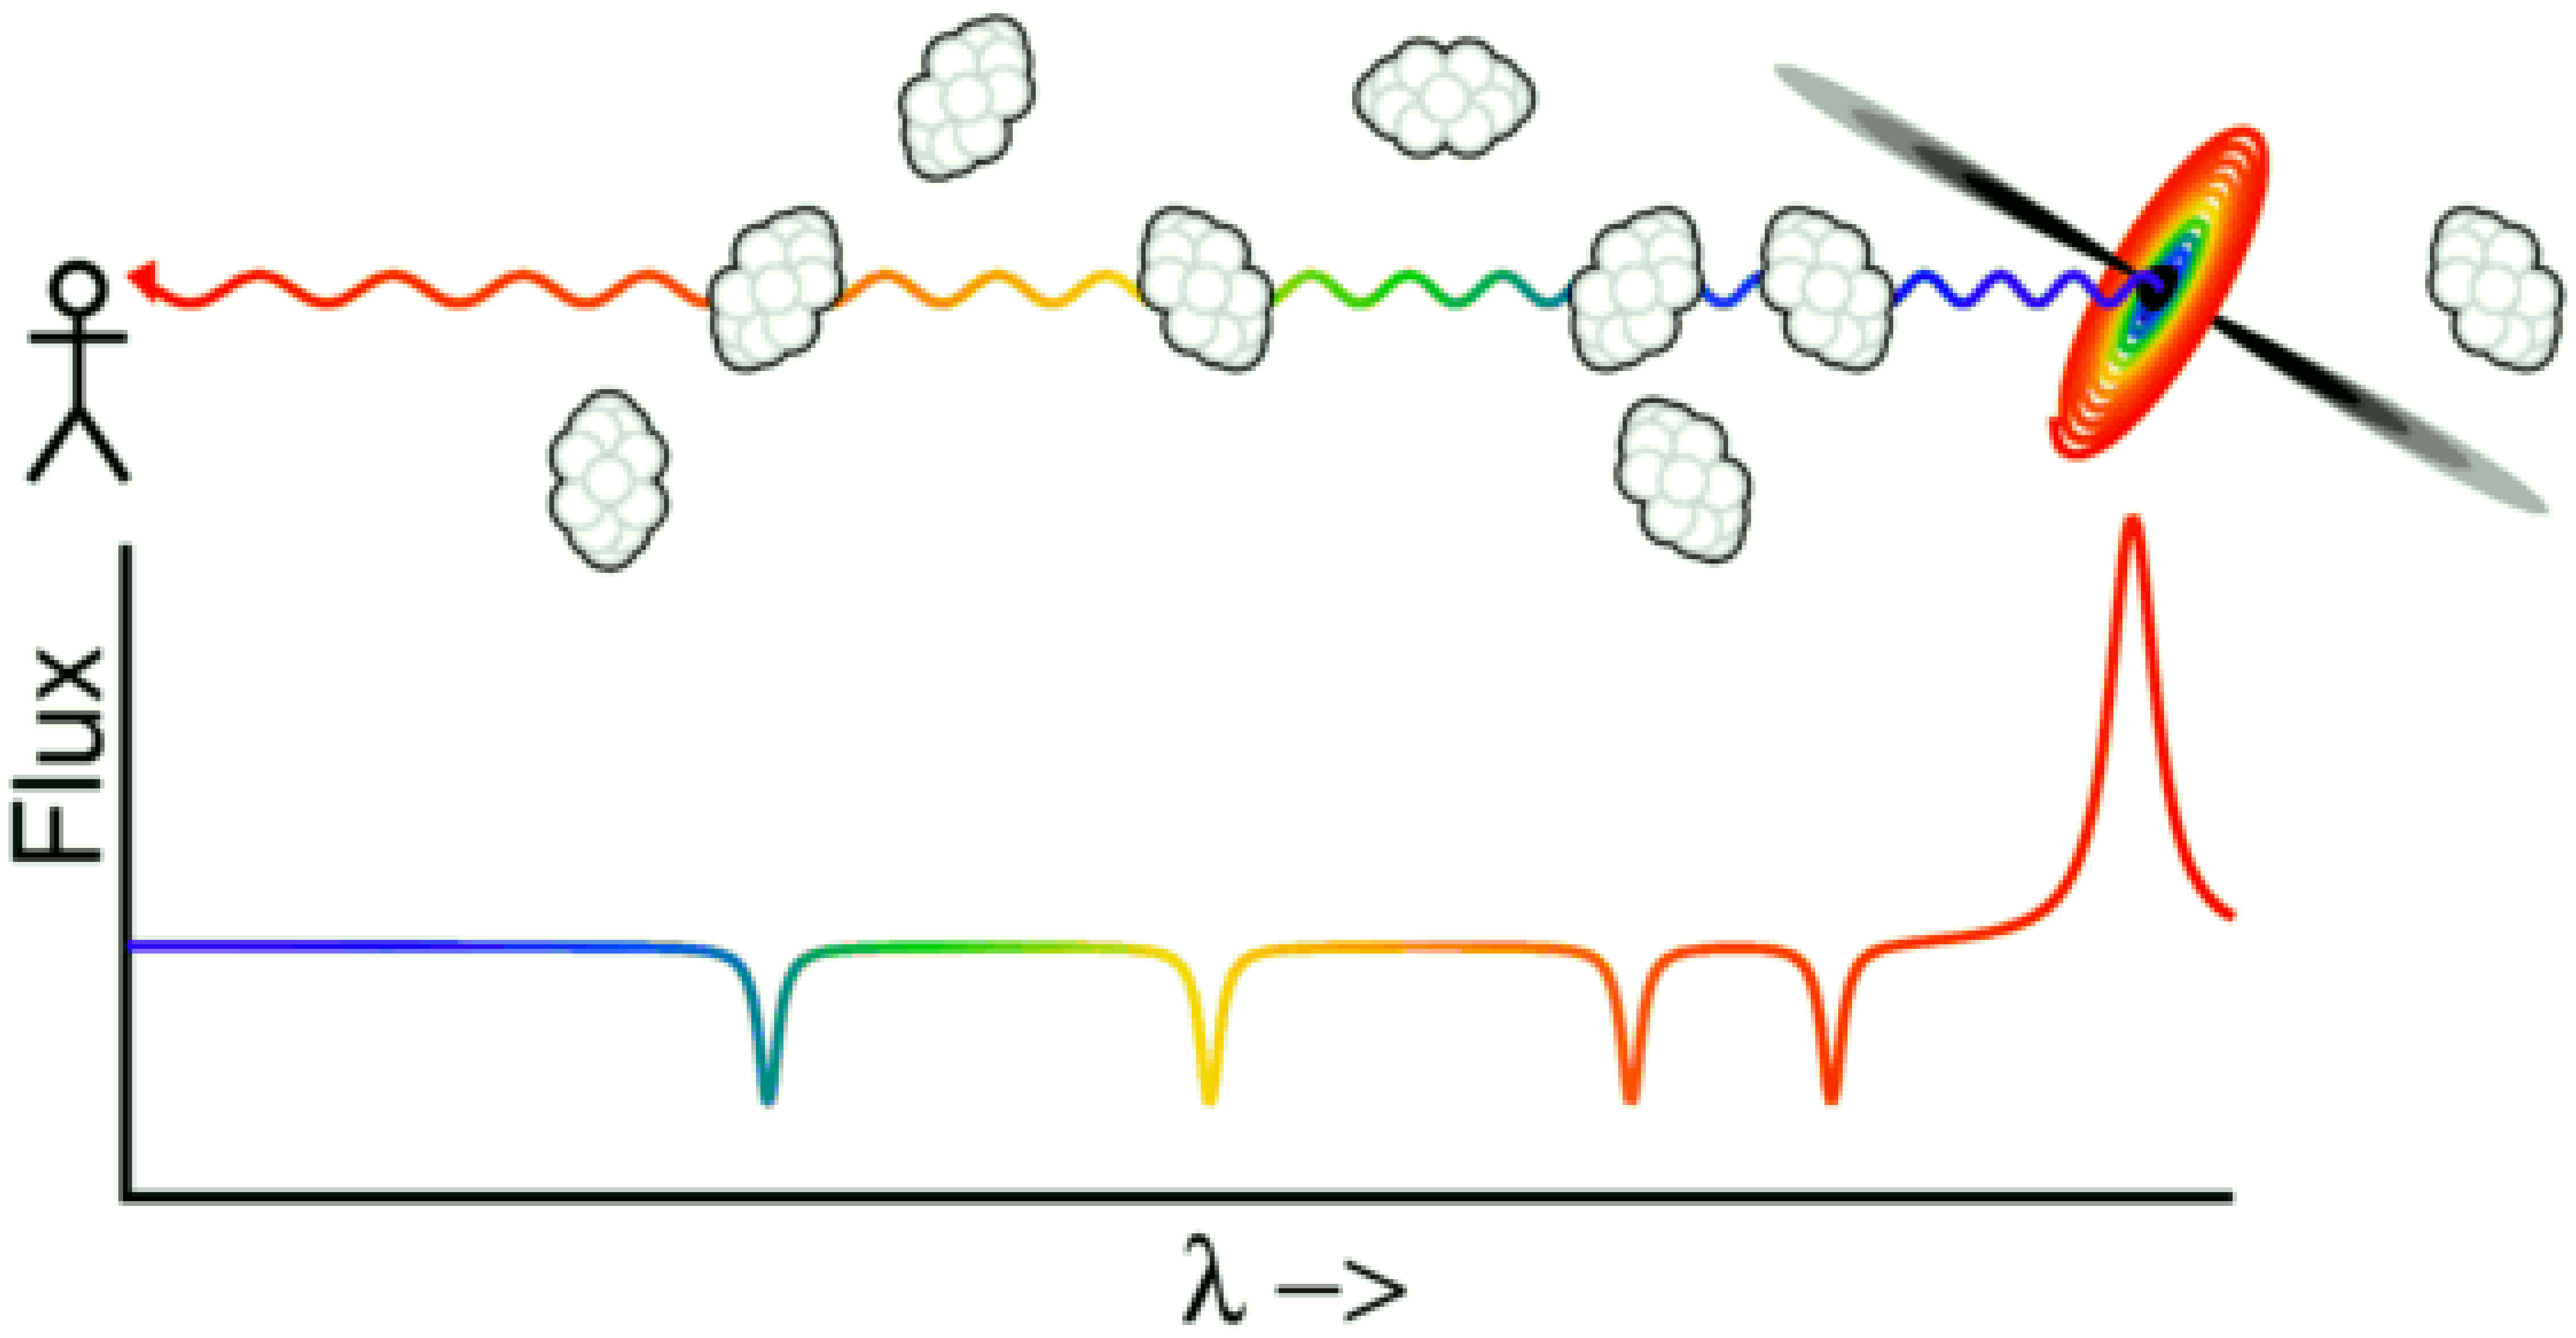
\includegraphics[width=12cm]{lyaf-75.eps}
  \caption{Illustration of the basic physics behind the \lya\ forest and how gas at different locations along the line of sight results in absorption lines at different wavelengths. (Image from {\tt http://www.astro.ucla.edu/})}
  \label{fig:LyaCartoon}
\end{figure}

The same logical progression also applies to the other lines in the Lyman-series. Therefore, you could imagine observing a \lyb\ and Ly\ $\gamma$\ forest at smaller wavelengths. There are a couple differences, however. First, lines deeper in the series have a smaller cross section for absorption, so intervening hydrogen will absorb less at these frequencies. Second, photons emitted from a background source with energies larger than \lyb\ will redshift through the \lyb\ wavelength and \textit{also} possibly through the \lya\ wavelength before reaching us and will have two opportunities to be absorbed. The photon's physical location when it redshifts through those two wavelengths will be completely different and, therefore, when observing absorption lines in the \lyb\ forest, it can be difficult to tell if the photons were absorbed by distant gas undergoing a \lyb\ transmission or closer gas undergoing a \lya\ transition. This problem is clearly exacerbated when considering higher-order lines since a larger number of distinct regions along the line of sight can contribute to the absorption.


We show two example quasar spectra in Figure \ref{fig:LyaExample}. The spectrum in the top panel is for a quasar at relatively low redshift and shows very little absorption. Meanwhile, the quasar in the bottom panel shows little absorption for emitted wavelengths redward of \lya\ but is heavily punctuated by absorption blueward of \lya\ due to intervening neutral hydrogen.
 
\begin{figure}[h]
  \centering
  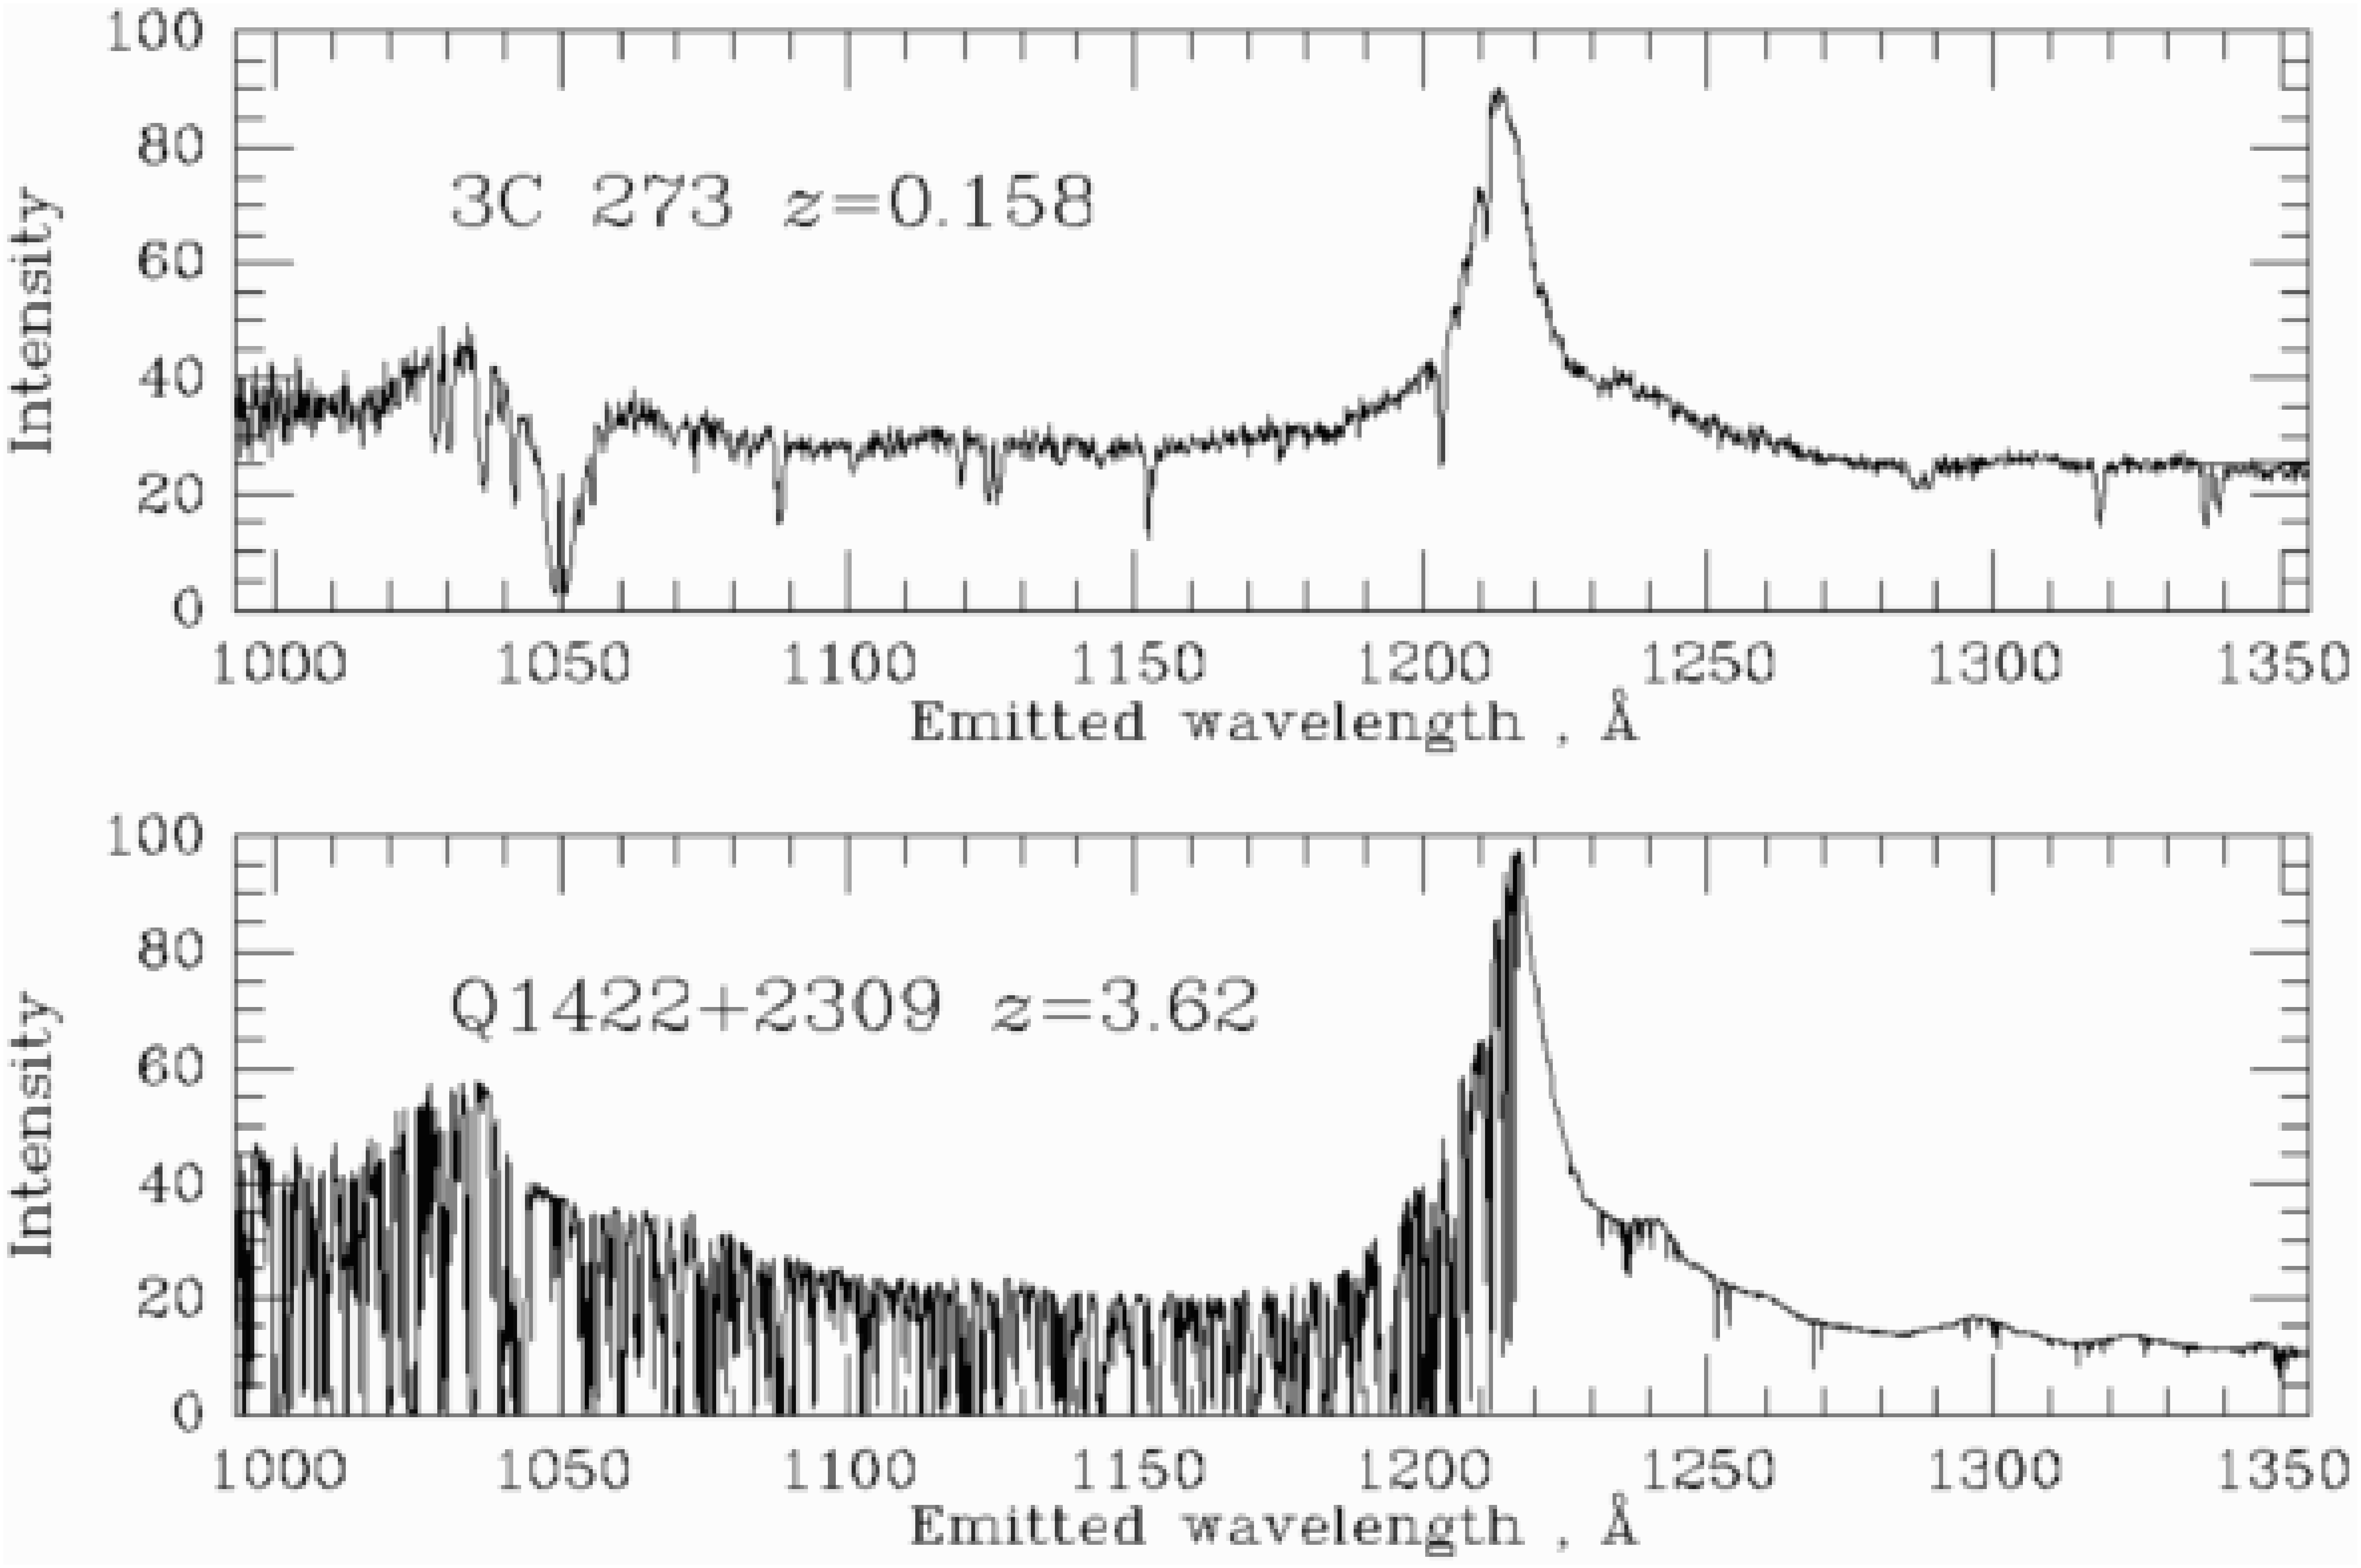
\includegraphics[width=12cm]{Lya-forest-60.eps}
  \caption{Flux as a function of rest-frame wavelength for a quasar at $z = 0.158$ (top) and $z = 3.62$ (bottom). The denser IGM at higher $z$ results in a dense ``forest" of absorption lines blueward of the rest-frame \lya\ line in the lower panel. (Image from {\tt http://www.astro.ucla.edu/})}
  \label{fig:LyaExample}
\end{figure}

At this point, the \lya\ forest should sound like a perfect tool: if we want to map the distribution of neutral hydrogen along the line of sight to a distant bright source, we can simply map each absorption line in the \lya\ forest to a parcel of neutral hydrogen. However, the story becomes complicated here due to the extremely large cross section for \lya\ absorption. Namely, the optical depth\nomenclature[Zp]{Optical Depth}{Optical depth, denoted by $\tau$, is a quantity that describes that likelihood for a photon to be absorbed, usually by a gas. The fraction of photons that will pass through the gas unabsorbed is $e^{-\tau}$.} for \lya\ absorption of a neutral hydrogen gas parcel is approximately

\begin{align}
\tau_{\alpha} &\approx 3.3 \times 10^{4} \xhi (1 + \delta) \left[\dfrac{1+z}{6.5}\right]^{3/2}. \label{eq:tauGP}
\end{align}

Using this expression, we can calculate the minimum neutral fraction needed for a gas parcel at mean density to allow 1\% transmission at $z = 5.5$:

\begin{align}
.01 &= e^{-\tau_{\text{min}}} \implies \tau_{\text{min}} \approx 4.6\\
4.6 &\approx \tau_{\alpha} x_{\text{HI,min}} \\
\implies x_{\text{HI,min}} &\approx 0.00014.
\end{align}


This reveals the fly in the ointment here: even a gas parcel that is 99.9\% ionized will allow less than 1\% transmission at the redshifts of interest for reionization. This allows absorption features to be caused by highly-ionized gas that happens to be over-dense. Therefore, we can not simply map absorption lines in the \lya\ forest to regions of significantly-neutral hydrogen. In fact, the second example quasar we see in Figure \ref{fig:LyaExample} shows significant \lya\ absorption and is located at $z = 3.62$, \textit{much later than the end of reionization}. At this point, the reader may ask what utility does the \lya\ forest have at all? Well, an enormous amount. To name a very few applications outside of reionization, since \lya\ absorption can be caused by matter overdensities, the \lya\ forest can be used to measure the matter power spectrum in the IGM. This, in turn, can be used to measure the baryon acoustic oscillations (BAO), provide lower limits on the mass of the dark matter (\citealt{Viel:2013fqw}), and constrain dark energy, for example. Additionally, absorption features due to damped \lya\ absorbers (DLAs) can be used to measure the primordial deuterium abundance as a test of big bang nucleosynthesis.\\
\textcolor{white}{suspense!}\\
\noindent But how to constrain the EoR?



\subsubsection{Evolution of $\tau_{\text{eff}}$}

% The Gunn-Peterson optical depth to \lya\ photons is \tau_{\text{GP}} = \dfrac{\pi e^2}{m_e c} f_{\alpha} \lambda_{\alpha} H^{-1}(z)n_{\text{HI}}

% Absorption is understood as being caused by the fluctuating Gunn-Peterson effect, low density regions in approximate thermal equilibrium between photoionization heating by the UV background and adiabatic cooling due to the Hubble expansion, rather than discrete \lya\ absorbers.

% By studying the evolution of the average transmitted flux or effective optical depth, one can trace the evolution in the 

% You probably want to re-read and refer to Lidz et al. that discuss that the evolution in the effective optical depth can be replicated by density fluctuations

Perhaps the most common analysis performed on high-redshift quasar spectra in the context of constraining the EoR is measurements of the effective Gunn-Peterson optical depth, defined as

\begin{align}
\langle F \rangle &\equiv e^{-\tau_{\text{eff}}}
\end{align}
\gloss{$\tau_{\text{eff}}$}{The effective Gunn-Peterson optical depth, which is the negative log of the mean transmission over a given redshift bin. Measurements of $\tau_{\text{eff}}$ are often converted into constraints on the photoionizaiton rate}where $\langle F \rangle$ is the averaged transmission fraction over a redshift bin in a quasar/GRB spectrum. Under the assumption of a uniform ionizing background and ionization equilibrium, where the rate that neutral hydrogen atoms are ionized is equal to the rate that ionized hydrogen atoms recombine, the effective optical depth encodes important information about the state of the IGM. In order to see this, we can take a few steps to express the optical depth in terms of the properties of the IGM.\footnote{The following discussion will borrow heavily from \cite{FaucherGiguere:2007jc} and \cite{fan2002evolution}.} First, the Gunn-Peterson optical depth can be expressed as

\begin{align}
\tau_{\text{GP}} &= \dfrac{\pi e^{2}}{m_{e} c} f_{\alpha}\lambda_{\alpha} \dfrac{n_{\text{HI}}}{H(z)}, \label{eq:tauGP}
\end{align}

where $H(z)$ is the Hubble parameter at redshift $z$, $e$ is the charge of the electron, $m_e$ is the electron mass, $c$ is the speed of light, $\lambda_{\alpha}$ is the \lya\ wavelength, $f_{\alpha}$ is the quantum mechanical oscillator strength, and $n_{\text{HI}}$ is the number density of neutral hydrogen atoms\gloss{HI}{Neutral hydrogen}\gloss{HII}{Ionized hydrogen}\gloss{HeI}{Neutral helium}\gloss{HeII}{Singly-ionized Helium}\gloss{HeIII}{Fully-ionized helium}\gloss{$f_{\alpha}$}{Quantum mechanical oscillator strength for the \lya\ transition}\gloss{$e$}{Charge of the electron}\gloss{$\lambda_{\alpha}$}{Wavelength of the \lya\ transition}\gloss{$m_e$}{Mass of the electron}. All of these quantities are known with the exception of the number density of neutral hydrogen atoms. To find this, we first utilize the statement of ionization equilibrium:

\begin{align}
\Gamma_{\text{HI}} n_{\text{HI}} &= R(T)n_{e}n_{\text{HII}} \label{eq:IonEquilibrium} \\
n_{\text{HI}} &= \dfrac{R(T) n_{e} n_{\text{HII}}}{\Gamma_{\text{HI}}} \label{eq:nH}\\
x_{\text{HI}} &= \dfrac{R(T)n_e}{\Gamma_{\text{HI}}} \label{eq:xHI}
\end{align}

where $\Gamma_{\text{HI}}$\gloss{$\Gamma_{\text{HI}}$}{Photoionization rate for hydrogen atoms. This depends on the number,  location, and properties of the ionizing sources.} is the photoionization rate due to the ionizing sources, $n_{e}$ is the number density of free electrons, $n_{\text{HII}}$ is the number density of ionized hydrogen atoms (protons), and $x_{\text{HI}}$ is the hydrogen neutral fraction. The left-hand side of Eq. \ref{eq:IonEquilibrium} represents the rate of photoionizations per volume and the right hand side represents the rate of hydrogen recombinations per volume. Under the assumption of ionization equilibrium with a uniform ionizing background, the presence of any transmission suggests $n_{\text{HII}} \approx n_{\text{HI}} + n_{\text{HII}} = n_{\text{H}}$ and 

\begin{align}
\bar{n}_{\text{H}} &= \frac{\rho_{c}(z)\Omega_{b}(z)X_{\text{H}}}{m_p} = \dfrac{3H^{2}(z)}{8\pi G} \dfrac{\Omega_{b}(z) X_{\text{H}}}{m_{p}} \\
&= \dfrac{3H_{0}^{2}\Omega_{b,0}}{8\pi G} \dfrac{X_{\text{H}}}{m_p}(1+z)^{3}\\
n_{\text{H}} &= (1+\delta) \bar{n}_{\text{H}}. \label{eq:ntot}
\end{align}

In this expression, $\rho_c$\gloss{$\rho_{c}$}{Critical energy density for a flat Universe} is the critical density for a flat Universe, $\Omega_{b}$\gloss{$\Omega_b$}{Baryon density in units of the critical density} is the baryon density in units of the critical density, $X_{\text{H}}$\gloss{$X_{\text{H}}$}{The fraction of baryonic mass in the form of hydrogen} is the fraction of baryonic mass in the form of hydrogen, $m_{p}$ is the mass of the proton which is effectively equal to the mass of the hydrogen atom, and $\delta \equiv (\rho-\bar{\rho})/\bar{\rho}$\gloss{$\delta$}{The local mass overdensity in units of the cosmic mean} is the local mass overdensity in units of the cosmic mean. A subscript of ``0" denotes that these are present-day values and $\bar{n}_{\text{H}}$ denotes the average of $n_{\text{H}}$. Thus, as we expect, this expression is essentially equal to the mass density of hydrogen atoms in the Universe divided by the mass per atom.\footnote{It may be interesting to note that this value corresponds to 4 hydrogen atoms per cubic meter today and roughly $\sim$1100 hydrogen atoms per cubic meter at $z = 5.5$. It is very empty out there.}  The expression for the electron number density should be the same, since each ionized hydrogen atom releases one free electron. However, it is probably the case that helium is singly ionized along with hydrogen, so the number density will increase according to:

\begin{align}
\bar{n}_e &= \bar{n}_{\text{H}} + \bar{n}_{\text{He}} = \dfrac{3H^2}{8\pi G}\left( \dfrac{X_{\text{H}}}{m_{p}} + \dfrac{(1 - X_{\text{H}})}{4m_{p}} \right) \\
&\approx 1.08 \bar{n}_{\text{H}}. 
\end{align}

However, for simplicity here, let us approximate $n_{\text{tot}} \equiv n_{e} \approx n_{\text{H}}$. The quantity $R(T)$ in Eq. \ref{eq:IonEquilibrium} is the recombination rate, which is equal to (\citealt{Hui1997}):

\begin{align}
R(T) &\approx 4.2 \times 10^{-13}\left( \dfrac{T}{10^{4} K}\right)^{-0.7} \text{cm}^{3}\sec^{-1}. \label{eq:RecombinationRate}
\end{align}

For $\delta \lesssim 5$, \cite{Hui1997} showed that the temperature and density follow the relationship

\begin{align}
T &\approx T_{0}(1+\delta)^{\gamma - 1} \label{eq:Trelation}
\end{align}

where $T_0$ is the temperature of a parcel of gas at mean density, and $\gamma$ is the slope of the temperature-density relation. For compactness, let's define $R_{4} \equiv R(T=10^{4}K)$. At this point, we are ready to combine Eq. \ref{eq:Trelation}, \ref{eq:RecombinationRate}, \ref{eq:ntot}, \ref{eq:nH}, and \ref{eq:tauGP} to get an expression for $\tau_{\text{GP}}$:

\begin{align}
\tau_{\text{GP}} &= \dfrac{\pi e^2}{m_e c}\dfrac{f_{\alpha}\lambda_{\alpha}}{H(z)} \dfrac{R_{4}(1+\delta)^{-0.7(\gamma - 1)}\bar{n}_{\text{tot}}^{2}(z)(1+\delta)^2}{\Gamma_{\text{HI}}}\\
&= \dfrac{\pi e^2}{m_e c}\dfrac{f_{\alpha}\lambda_{\alpha}}{H(z)} \dfrac{R_4 \bar{n}_{\text{tot}}^{2}(z)}{\Gamma_{\text{HI}}} (1+\delta)^{2-0.7(\gamma-1)}. \label{eq:tauGPfinal}
\end{align}

Finally, we have an expression for the \lya\ optical depth in terms of several properties of the IGM. The primary unknown in the above expression is the photoionization rate, which is a very complicated parameter which depends on the number, intensity, spectrum, and proximity of ionizing sources among other things. A common assumption in these types of analyses is that the photoionization rate is approximately spatially uniform. This seems like a plausible assumption in a post-reionization Universe, when the mean free path of ionizing radiation is long allowing any given gas parcel can receive ionizing radiation from many sources. On the other hand, early in reionization, the Universe is opaque to ionizing radiation and gas parcels tend to only see sources within their own ionized regions. Regardless, with this approximation, the observed mean transmission in a region of the spectrum is akin to an average of Eq. \ref{eq:tauGPfinal} marginalizing over the density field:

\begin{align}
\left\langle F \right\rangle &= \int \dd \delta\ e^{-\tau(\delta)} P(\delta) \equiv e^{-\tau_{\text{eff}}}.
\end{align}


 As such, an intriguing question is, if you have a model for the probability distribution of the underlying density field, what (uniform) value of $\Gamma_{\text{HI}}$ will yield a value for $\left\langle F \right\rangle$ that is consistent with observations? This question has received a lot of attention ({\bf cites}) and has led to many measurements of the photoionization rate. With estimates of the photoionization rate in hand, we can utilize Eq. \ref{eq:xHI} in order to obtain measurements of the IGM neutral fraction in each redshift bin in the spectra in order to gauge the progress of the EoR. Results for measurements of $\Gamma_{\text{HI}}$ and $\axhi$ via this method, performed by \cite{Fan2006a}, are shown in Figure \ref{fig:tauEffResults}. This figure demonstrates that, using $\tau_{\text{eff}}$ and the assumption of ionization equilibrium, estimates of the neutral fraction are exceedingly small for $z \lesssim 6$. This argument has played a large part in forming the common knowledge that reionization has ended by $z = 6$. 

\begin{figure}[h]
  \centering
  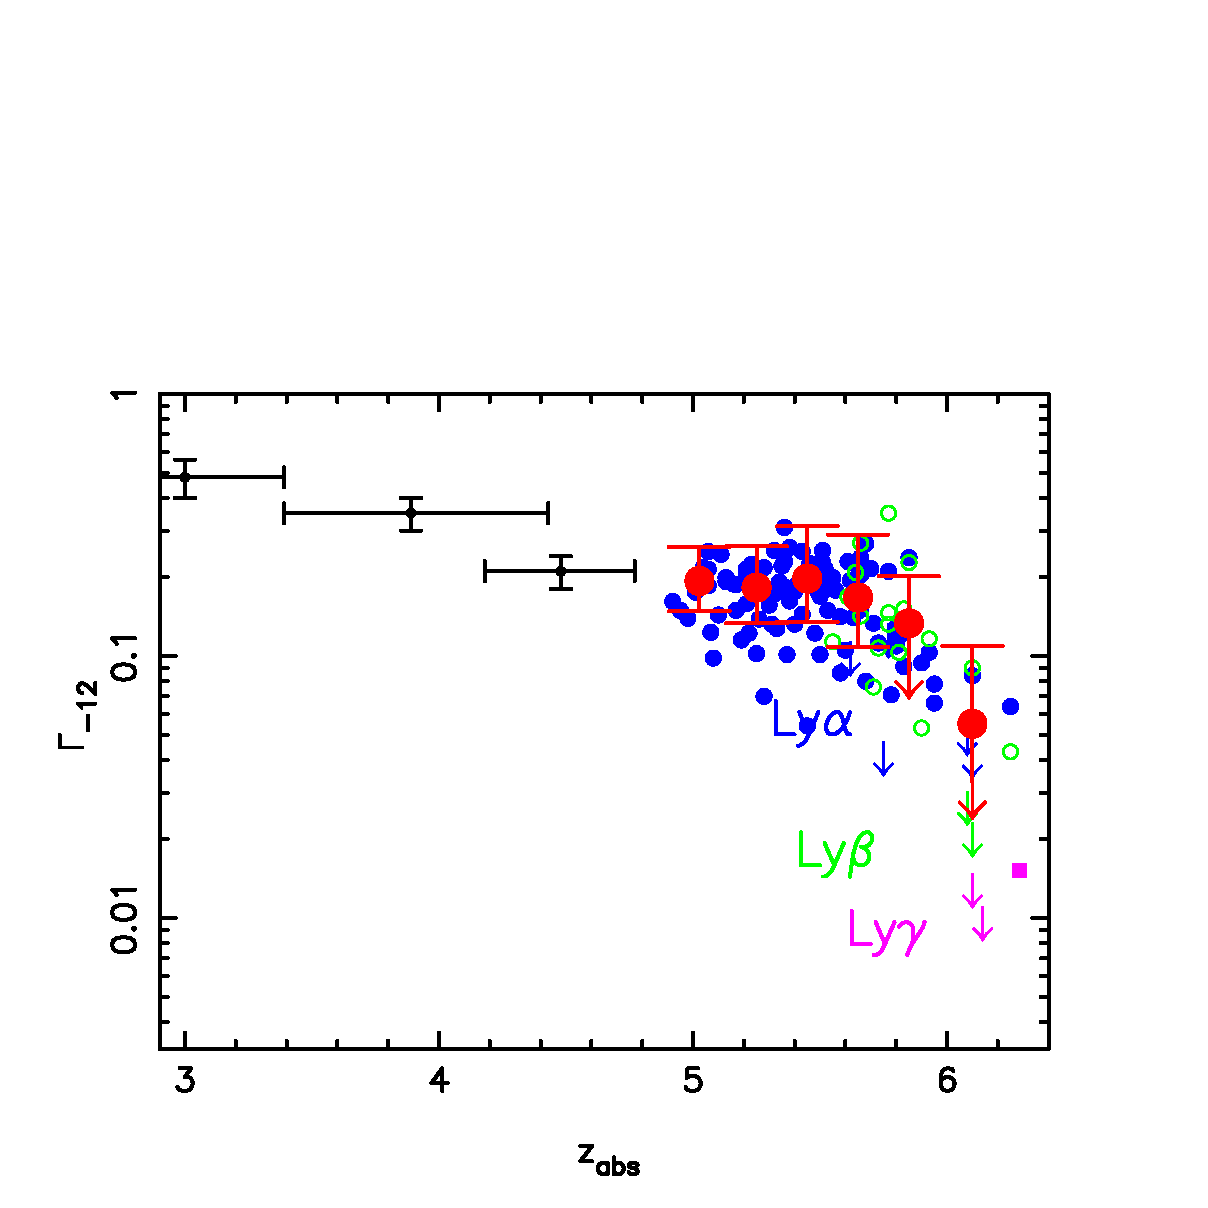
\includegraphics[width=8cm]{Fan.gamma.eps}
  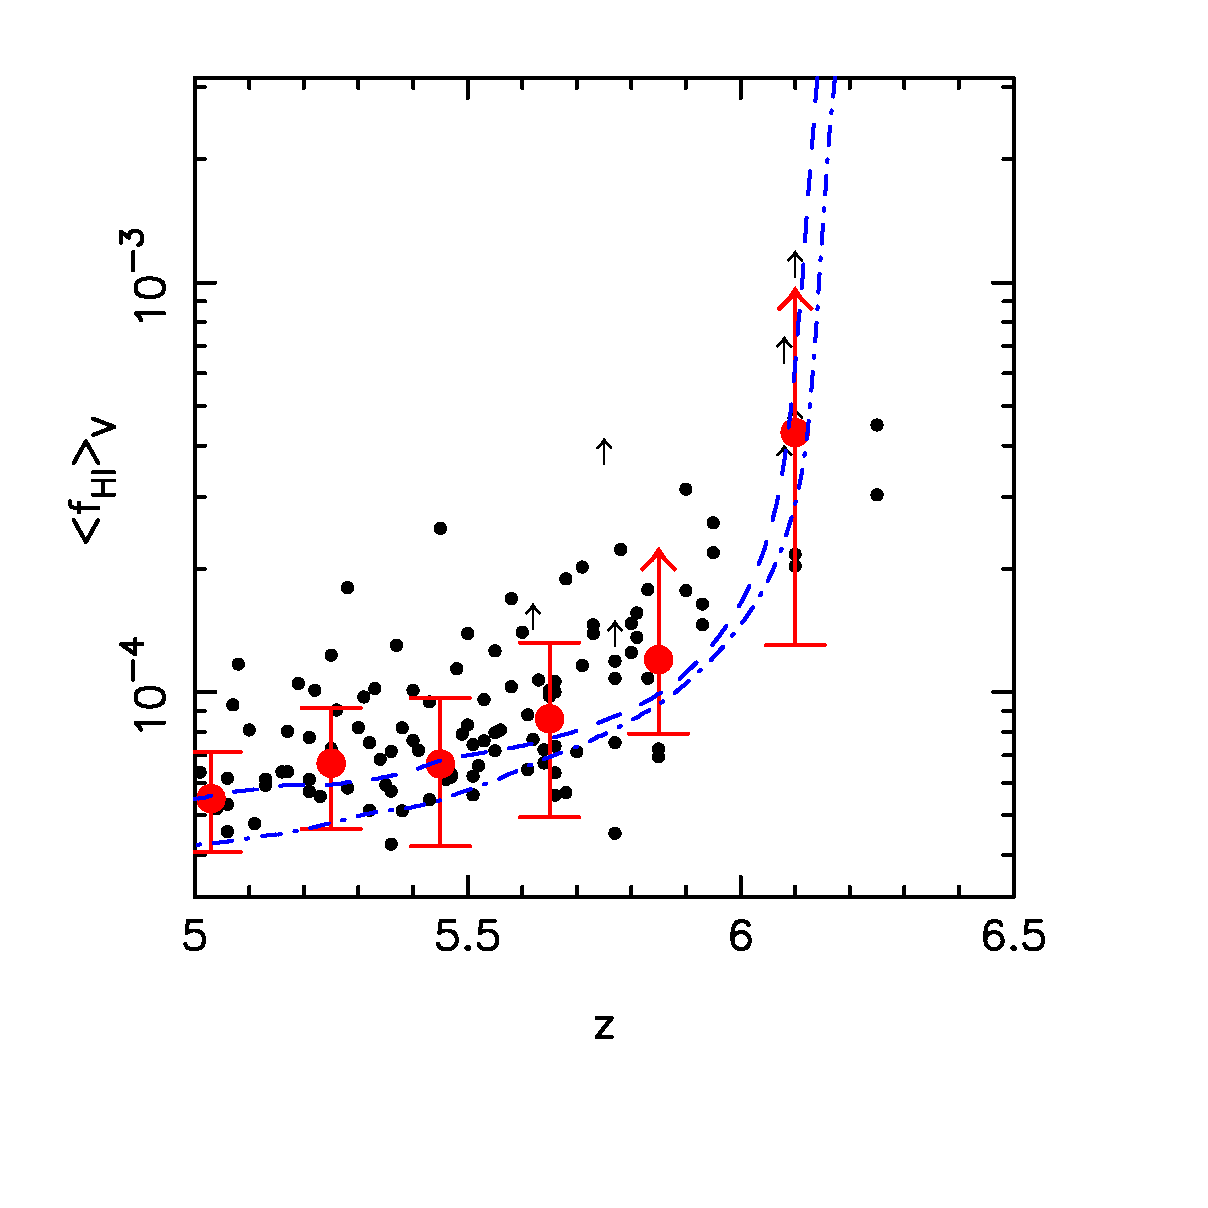
\includegraphics[width=8cm]{Fan.fHv.eps}
  \caption{Measurements of $\Gamma_{\text{HI}}$ (top) and $\axhi$ from \cite{Fan2006a} (bottom).}
  \label{fig:tauEffResults}
\end{figure}


Despite the widespread analysis of $\tau_{\text{eff}}$ in constraining the end of reionization, the interpretation of $\tau_{\text{eff}}$ is quite complicated.\footnote{For a more thorough discussion of controversial aspects of these constraints, see the intro for \cite{McGreer:2011dm}.} First, accepting the assumption of the IGM being in ionization equilibrium with a uniform $\Gamma_{\text{HI}}$ is tantamount to assuming that reionization has ended. Specifically, as discussed in \S \ref{sec:CosmicContext}, reionization is likely a highly inhomogeneous process with ionized bubbles forming around the brightest sources, growing, and eventually overlapping. During the period prior to complete overlap, regions of neutral hydrogen will be shielded from the ionizing radiation while ionized bubbles will experience a very large $\Gamma_{\text{HI}}$. This is not reflected in Eq. \ref{eq:IonEquilibrium} and so we expect conclusions derived from this method to be unreliable when we begin to push up against the end of reionization. Additionally, interpretation of the level of flux in quasar spectra in the context of reionization is further complicated by the fact that quasars likely reside in very atypical parts of the Universe. Specifically, \cite{Lidz:2007mz} show that it is likely that some quasar lines of sight will pass through mostly ionized gas even up to neutral fractions of $\axhi \sim 0.5$. 

%\subsubsection{Dark Gap Sizes}
%
%Yeah, so the main point we want to (briefly) drive home here is that previous constraints on $\axhi$ from the use of dark gap statistics probably assumed a uniform $\Gamma_{\text{HI}}$, which is equivalent to assuming reionization has already ended anyway. 
%
%Fan says imperfect sky subtraction in regions with strong OH lines can cause significant residuals resulting in an \textit{underestimate} in the dark gap size. Although, it seems like they don't allow any room for noise fluctuations in what they constitute a dark gap???


\subsubsection{Dark Pixel Covering Fraction}

As demonstrated in the previous section, interpreting measurements of the effective optical depth in the context of reionization is complicated and can rely on controversial assumptions. However, an alternative approach is to consider what constraints can be made without resorting to such assumptions. In this regard, an important method in estimating $\axhi$ from high-redshift quasar observations is the dark pixel covering fraction. This approach is rooted in the fact that neutral parcels of gas are certain to result in saturated absorption in quasar spectra due to their optical depths being $\tau_{\text{HI}} \gtrsim 10^4$ (Eq. \ref{eq:tauGP}). Therefore, a reliable upper bound on the neutral fraction at a given redshift can be estimated by the fraction of pixels in quasar spectra that are completely absorbed at that redshift. 

An obvious drawback of this method is that, at $z \sim 6$, overdense yet ionized regions will also result in saturated absorption and will significantly increase this upper bound on the neutral fraction. One approach to combat this effect is to incorporate the \lyb\ forest into the analysis. The optical depth for Lyman-series transitions scales as $f\lambda$, where $f$ is the oscillator strength of the transition and $\lambda$ is the corresponding wavelength. Therefore, the analogous expression of Eq. \ref{eq:tauGP} for \lyb\ is:

%Useful quantities:                                                                                                   
% Oscillator Strengths                                                                                                
% f_21 = 0.4162 (1s-2p)  lambda_21 = 1215.67 AA                                                                       
% f_31 = 0.0791 (1s-3p)  lambda_31 = 1025.72 AA                                                                       
% f_32 = 0.4349 (2s-3p)  lambda_32 = 6562.74 AA 
\begin{align}
\tau_{\beta} &= \tau_{\alpha} \times \dfrac{f_{\beta}\lambda_{\beta}}{f_{\alpha}\lambda_{\alpha}} \approx 5.3 \times 10^{3} \xhi (1 + \delta) \left[\dfrac{1+z}{6.5}\right]^{3/2}. \label{eq:tauGPB}
\end{align}

where $f_{\alpha} = 0.4162$, $\lambda_{\alpha} = 1216 \AA$, $f_{\beta} = 0.0791$, and $\lambda_{\beta} = 1026\AA$. From this expression, we can see that a mean-density parcel of neutral gas should cause saturated absorption in both the \lya\ and \lyb\ transitions. Meanwhile, ionized overdense regions are less likely to cause saturated absorption as their optical depth in \lyb\ is reduced by a factor of $f_{\beta}\lambda_{\beta}/f_{\alpha}\lambda_{\alpha} \approx 1/6$. Therefore, limits from the dark-pixel covering fraction may be improved by requiring simultaneous absorption in both \lya\ and \lyb\ as part of the definition of a dark pixel. Additionally, the \lyb\ dark pixel covering fraction on its own is a viable tool for establishing an upper bound on the neutral fraction, although foreground \lya\ absorption may undo some of the gains from the lower $\tau_{\beta}$ value. In practice, all three approaches (requiring \lya, \lyb, and \lya +\lyb\ absorption) are used. 

This procedure faces several complications when actually carried out, however. First, quasar observations are subject to the noise from the night sky which effectively adds mean-zero random noise to the spectra. The addition of this random noise can result in spurious transmission in pixels that otherwise would have been completely absorbed. Therefore, to measure the dark pixel fraction in quasar spectra, one first needs to create a suitable definition of what qualifies as a ``dark" pixel. One approach here is to define dark pixels as having transmission below some threshold defined in terms of the noise standard deviation, $\sigma_{\text{N}}$. This presents us with a tradeoff, however, since larger thresholds will reduce the number of neutral pixels we miss but also increase the number of ionized pixels that get incorporated into the dark pixel population. Alternatively, if we are presented with median-zero noise, then half of all truly-absorbed pixels will result in negative flux values, on average. This presents the possibility of using twice the negative-flux-pixel covering fraction as an estimate of the dark-pixel covering fraction (or four times, in the case of requiring \lya +\lyb\ absorption) (\citealt{McGreer:2014qwa}). 

A second complication is that, since pixels have a finite width, their transmission values effectively represent an average of the transmission over some region in the spectra. If the pixel width is large enough, then it is possible for a pixel to have non-zero transmission despite corresponding to a physical region that contains significantly-neutral gas. For example, if the physical region in space associated with the pixel is 80\% composed of completely-neutral gas and 20\% composed of completely ionized gas which allows full transmission, then the transmission of that pixel will be 20\% and will likely not qualify as a ``dark pixel" despite containing neutral gas. Thus, even in a measurement as seemingly-simple as the dark-pixel covering fraction, these details must be kept in mind when interpreting results. 

Regardless, \cite{McGreer:2011dm} and \cite{McGreer:2014qwa} apply the dark-pixel covering fraction approach to 22 high-redshift quasar spectra to produce the constraints on $\axhi$ shown in Figure \ref{fig:McGreer}. Dimly-colored points correspond to \cite{McGreer:2011dm} while bold-colored points correspond to \cite{McGreer:2014qwa}. These results present a very different interpretation than using $\tau_{\text{eff}}$ measurements while using the same data. Namely, that model-independent constraints have a hard time conclusively confirming the common knowledge that reionization has ended by $z \sim 6$.\footnote{The authors here do go on to focus on a high-resolution subset of their quasar observations presented in \cite{McGreer:2014qwa} in order to argue in favor of an end to the EoR by $z \sim 6$. However, the precise interpretation of the spectra is complex, as discussed herein.} 

\begin{figure}[h]
  \centering
  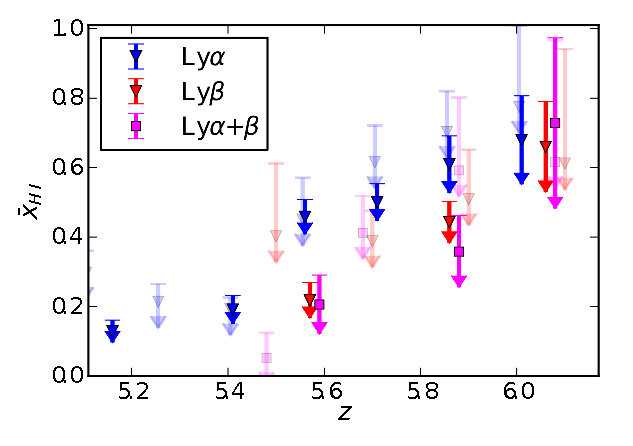
\includegraphics[width=8cm]{xhi_newdata.eps}
  \caption{Current limits on $\axhi$ derived from the dark-pixel covering fraction in \cite{McGreer:2014qwa}. Lightly-shaded points are older limits obtained in \cite{McGreer:2011dm}.}
  \label{fig:McGreer}
\end{figure}



\subsubsection{Damping Wing Redward of \lya}\label{sec:IntroDampingWing}

Much of the difficulties in using the \lya\ forest to constrain the timing of the EoR can be boiled down to the following problem: interpreting \lya\ absorption in high-redshift quasar spectra is difficult because both neutral and ionized gas can result in saturated absorption. Therefore, it is worth asking if there are any ways to break this degeneracy in \lya\ absorption in order to determine which absorption is likely due to neutral hydrogen. One potential approach toward this goal, which has received much attention (\citealt{Chornock:2013una}, \citealt{Chornock:2014fva}, \citealt{Mortlock2011}, \citealt{Bolton:2011vb}), is looking for the hydrogen damping wing redward of the \lya\ line. 


To understand this approach, let us first understand what the hydrogen damping wing is. For many applications, it is suitable to consider an atom's ability to absorb radiation as a series of delta functions in frequency: when incident radiation has a frequency exactly coinciding with the energy of the transition, then there is a non-zero probability for absorption and zero probability otherwise. In reality, the probability of absorbing a photon of a given frequency, e.g., the line profile, is a continuous distribution which, while small for frequencies $\nu \neq \nu_{0}$, is non-zero. 


The intrinsic line profile for the \lya\ transition in the hydrogen atom can be seen as arising from the time/energy uncertainty principle, $\Delta E \cdot \Delta t \gtrsim \hbar$. Specifically, the finite lifetime of the $n = 2$ excited state implies the existence of a range of energies that can excite, or result from, the transition. The distribution of this range of energies follows a Lorentzian distribution\gloss{Lorentzian Distribution}{Probability distribution for the ratio of two standard-normal-distributed variables. This distribution also describes the intrinsic line profile for absorption lines.}:\footnote{A quantum-mechanical discussion of this result can be found in \S 5.8 of \cite{sakurai2011modern}. A classical derivation can be found in \S 3.6 of \cite{rybicki1979radiative}.}

\begin{align}
\phi(\nu) &= \frac{1}{\pi} \dfrac{\Gamma/4\pi^{2}}{(\nu - \nu_{0})^{2} + (\Gamma/4\pi)^2}
\end{align}

with the corresponding absorption cross section

\begin{align}
\sigma_{\alpha}(\nu) &= \dfrac{\pi e^2}{m_{e}c} f_{\alpha} \phi(\nu). \label{eq:IntroLineProfile}
\end{align}

The ``damping wing" refers to the $\sigma \sim 1/(\nu-\nu_{0})^{2}$ behavior far from line center. This can be used to break the degeneracy between HII absorption and HI absorption because the optical depth is so much smaller in the damping wing that, without significantly-neutral gas (optical depth scales with neutral fraction), the optical depth at such frequency separations will not be sufficient to cause absorption. Furthermore, the damping wing has a distinct shape which can be fit for in order to infer the properties of the neutral gas which sources it. 


While the damping wing from an isolated neutral region in a sea of fully-ionized, $\tau = 0$ hydrogen would stand out like a sore thumb, in reality absorption from the surrounding dense, yet ionized, gas will punctuate the damping wing with additional absorption features and will make it harder to detect. This makes the prospect of looking for isolated damping wings in typical regions in quasar spectra unappealing. However, photons emitted slightly \textit{redward} of \lya\ cannot be absorbed by dense ionized gas since ionized gas has a negligible optical depth for $\nu \neq \nu_{\alpha}$. Neutral hydrogen, on the other hand, \textit{will} allow absorption to take place redward of \lya\ due to the significant optical depth in the damping wing. Because of this, searches for the damping wing slightly redward of the \lya\ line will be able to avoid nuisance absorption from neighboring ionized gas.


We show a famous example of a potential damping-wing detection in Figure \ref{fig:Mortlock}, taken from \cite{Mortlock2011}. This shows a region of the transmission spectrum for a quasar at redshift $z = 7.085$ (ULAS J1120+0641). The fractional transmission nearby the \lya\ line exhibits a gradual recovery from almost complete absorption at $\lambda < \lambda_{\alpha}$ to almost complete transmission at $\lambda > \lambda_{\alpha}$, occurring over a wavelength interval consistent with a hydrogen damping wing. The curves in blue show models for damping wing absorption associated with an IGM with neutral fraction $\axhi = 0.1$ (top), 0.5 (middle), and 1 (bottom) with a sharp ionization front at a distance of 2.2Mpc from the quasar. In green, a model for the absorption profile of a Damped \lya\ Absorber (DLA, see glossary for definition)\gloss{DLA}{Damped \lya\ Absorber. These are dense, isolated clouds of gas with extremely high column densities of neutral hydrogen, $N_{\text{HI}} \gtrsim 2\times10^{20}\cm^{-2}$ sufficient to exhibit damping-wing absorption. These are thought to source galaxy formation and are not part of the diffuse IGM which we want to study for reionization purposes.} with column density $N_{\text{HI}} = 4\times10^{20}\text{cm}^{-2}$ located 2.6 Mpc from the quasar is shown. Thus, the transmission profile appears consistent with both a significantly-neutral ($\axhi > 0.1$) IGM or a proximate DLA. However, \cite{Simcoe} perform a search for metal lines, which typically accompany DLA absorption, and find that the gas is extremely metal-poor. This bolsters the claim that the damping-wing absorption seen in this example is, in fact, due to diffuse neutral hydrogen in the IGM. 


\begin{figure}[h]
  \centering
  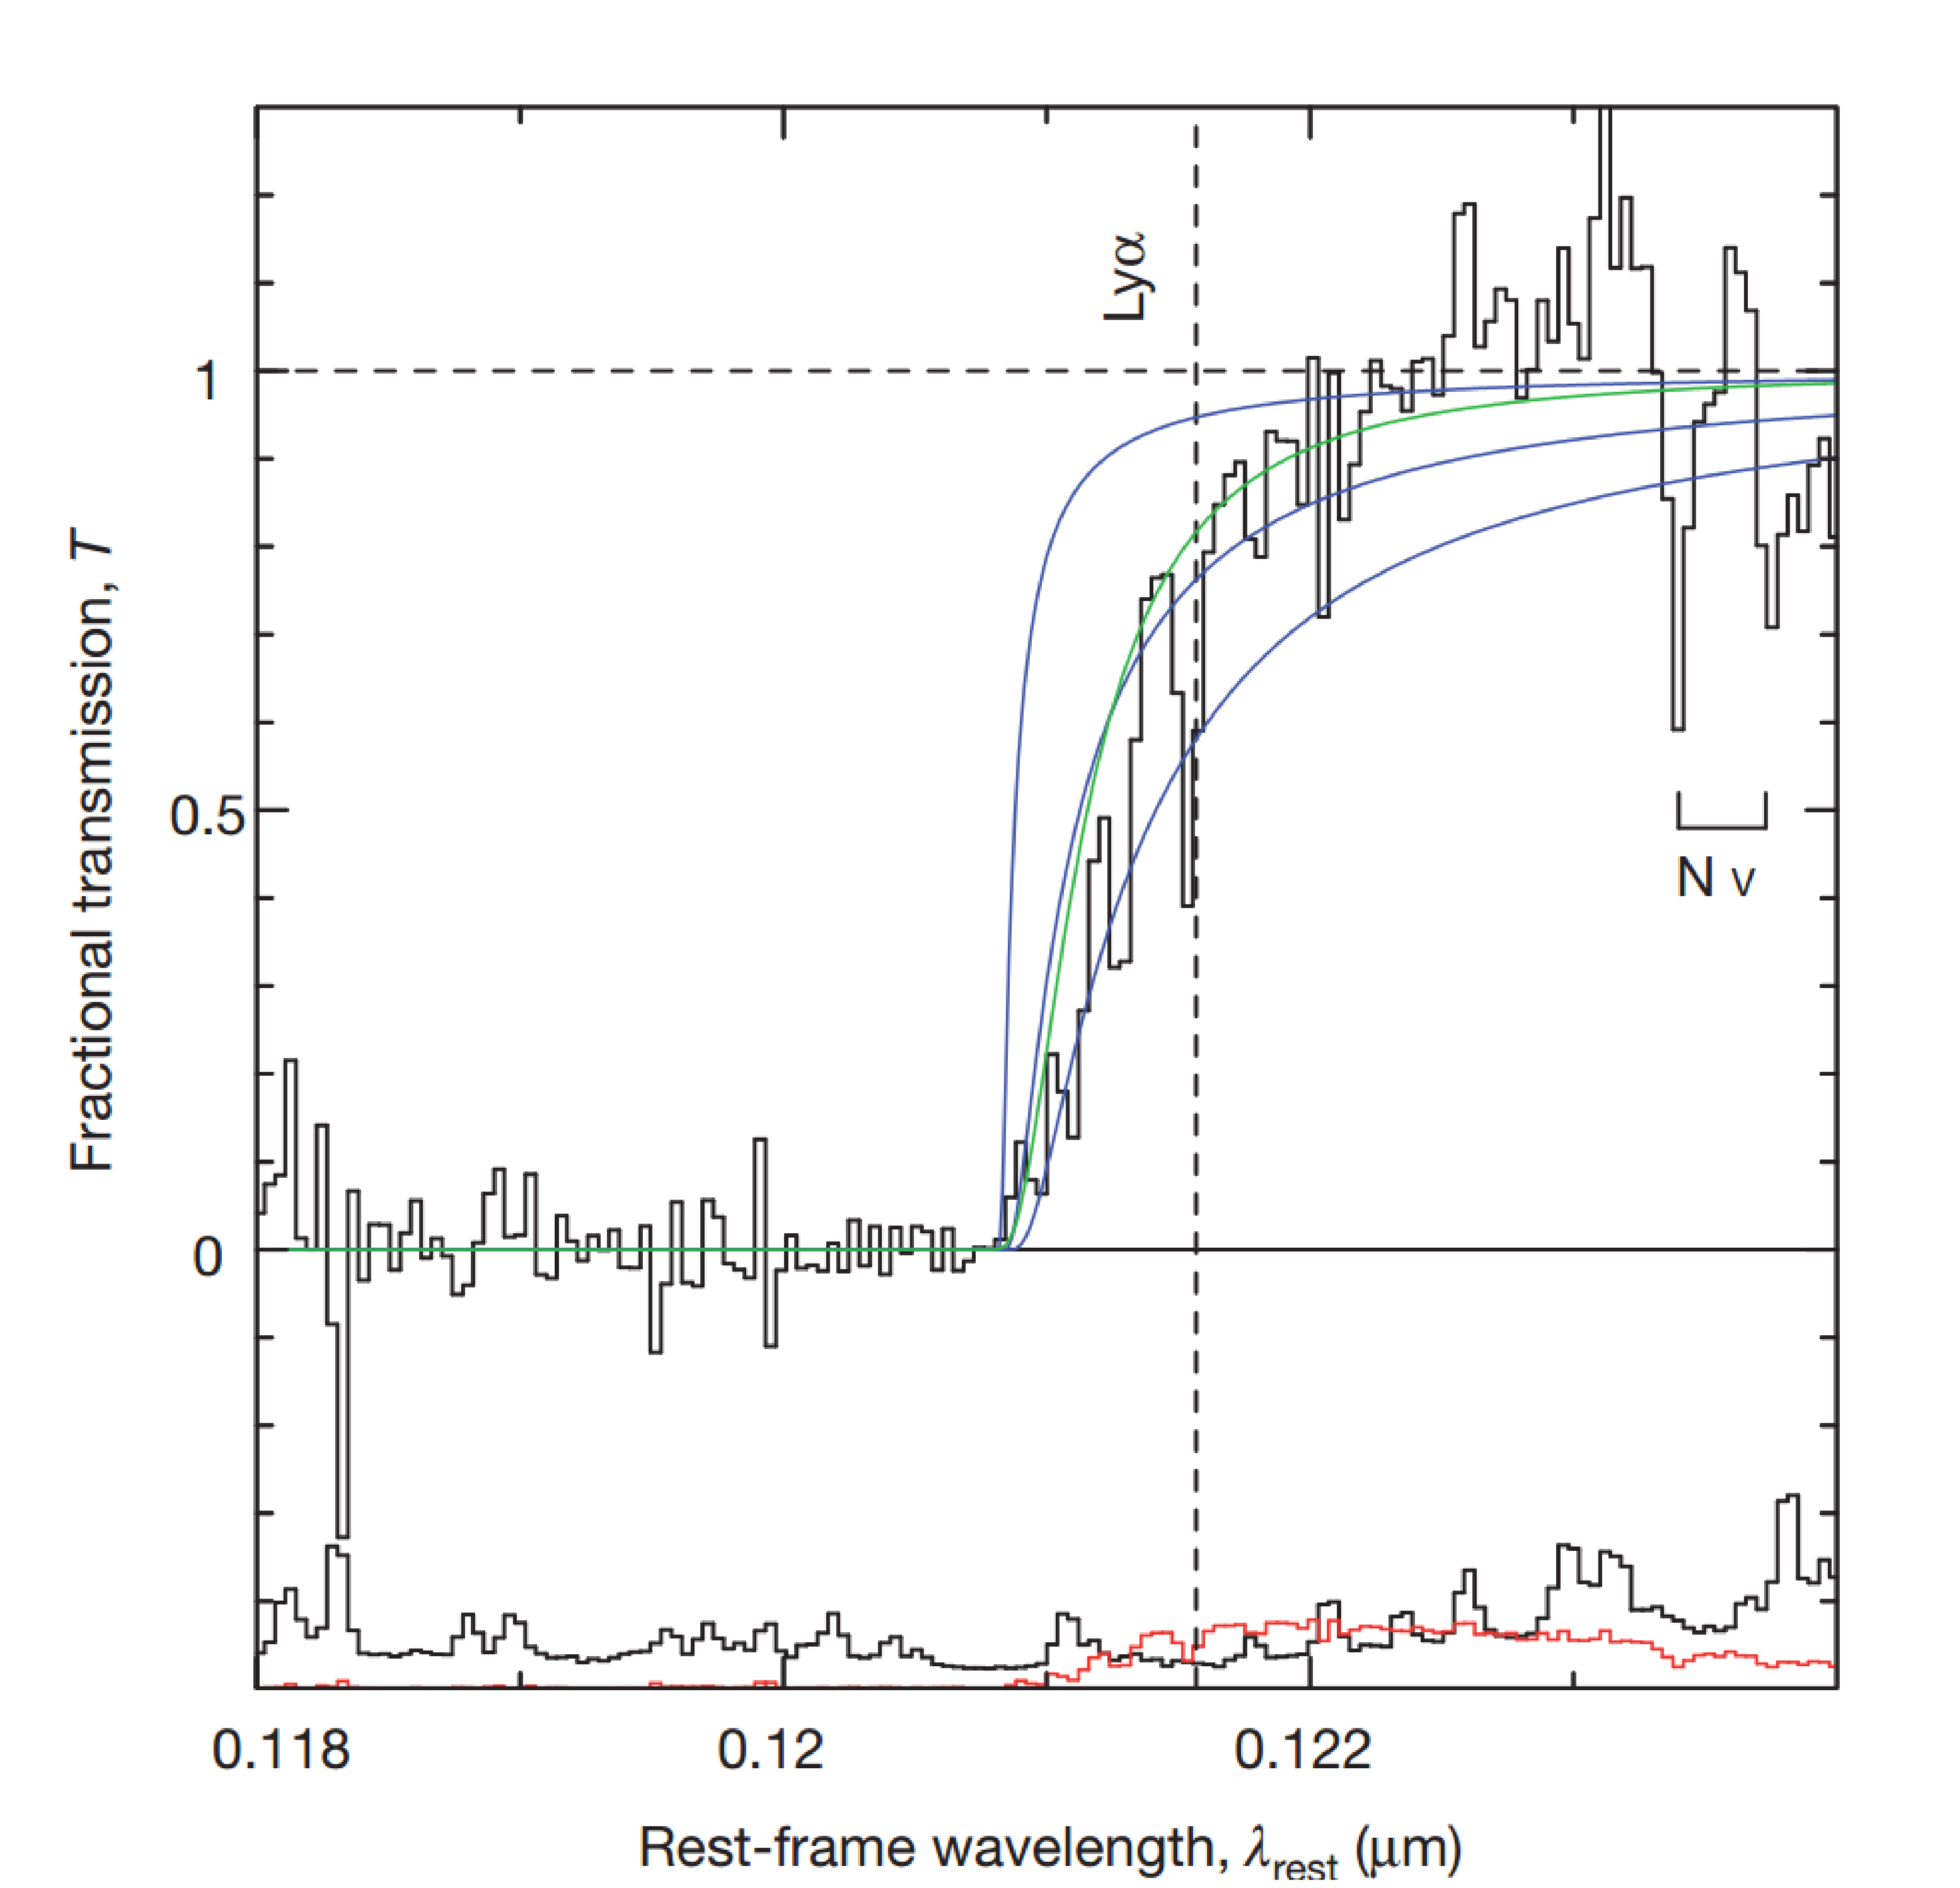
\includegraphics[width=8cm]{z7p085_DampingWing.eps}
  \caption{Quasar ULAS J1120+0641 identified at redshift $z = 7.085$ along with several fits for the damping wing.}
  \label{fig:Mortlock}
\end{figure}


Other searches for damping-wing absorption redward of \lya\ have been carried out on, for example, GRB 130606A (\citealt{Chornock:2013una}) and GRB 140515A (\citealt{Chornock:2014fva}). These authors looked for the damping wing in the spectra of GRB afterglows at redshift $z = 5.913$ and $z = 6.33$, respectively. A non-detection in the spectra of the $z = 5.913$ GRB allowed the authors to place a $2\sigma$ limit on the nearby IGM neutral fraction of $\axhi < 0.11$. Similarly, no strong evidence of a damping wing was found in the spectrum of GRB140515A, shown in Figure \ref{fig:GRB140515A}. The right-hand panel shows the transmission fraction nearby the \lya\ transition, which is equally-well fit by pure host absorption (blue, $N_{\text{HI}} = 10^{18.62}\text{cm}^{-2}$), pure IGM absorption from gas at $6.0 \leq z \leq 6.328$ with $\axhi = 0.056$ (red), and a hybrid model with a host absorber lying within an ionized bubble with $R = 10$ comoving Mpc met by an IGM with $\axhi = 0.12$ (green). As such, they argue against a significantly-neutral IGM at this redshift.  

\begin{figure}[h]
  \centering
  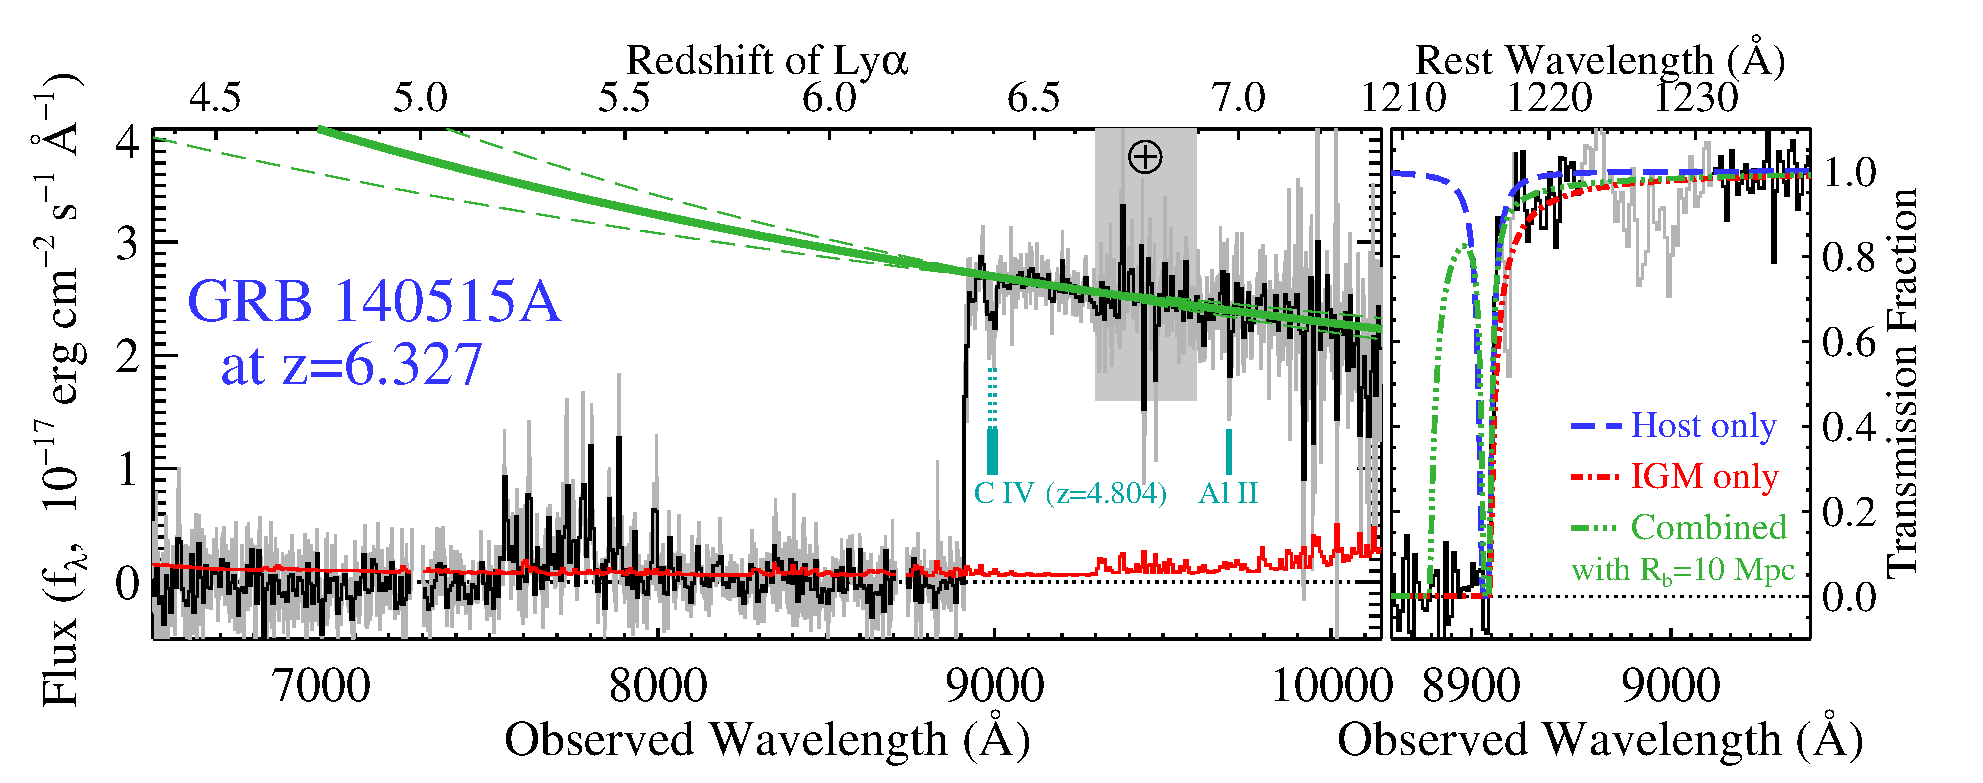
\includegraphics[width=14cm]{GRB140515A.eps}
  \caption{Spectrum of GRB140515A, a gamma-ray burst located at $z = 6.33$. The right-hand panel overlays damping wing models from a host absorber (blue), a pure IGM model with $\axhi = 0.056$ (red), and a combination model (green). The authors argue that, while each curve provides an equally-good fit to the data, the sharp rise in transmission shown is inconsistent with a significantly-neutral IGM. }
  \label{fig:GRB140515A}
\end{figure}


It is worth pointing out, however, that the method of searching for the damping wing redward of \lya\ is not without drawbacks. First, detecting the damping wing redward of \lya\ relies on your ability to understand what the quasar flux \textit{would have} been in the absence of the absorbing gas nearby the \lya\ line (this unabsorbed flux is referred to as the quasar \textit{continuum} and predicting the unabsorbed flux for a given quasar is called \textit{continuum fitting}). Predicting the \lya\ line properties in quasars is notoriously complicated and so modelling the precise fractional transmission must be done with care. Second, searching for the damping wing redward of \lya\ inherently involves measuring the gas properties nearby the quasar. However, quasars are extremely rare and special objects and it is not obvious that their surroundings are representative of the IGM on average. For example, \cite{Lidz:2007mz} found that quasars are likely born into large galaxy-generated ionized regions, suggesting that interpreting the \textit{lack} of a damping wing detection is not straightforward. Gamma-ray burst spectra are gaining attention in this regard (See \citealt{Salvaterra:2015gpa} for a review) as they tend to occupy more typical regions of space and have an easier-to-model continuum flux. The drawbacks of GRBs, though, is that they are often accompanied by a host absorber whose damping-wing absorption must be separated from that of the IGM. Third, even when provided with a clean detection of the damping wing redward of \lya, this will only tell you about one region of space and it will be difficult to use this single observation to extrapolate to the ionization state of the IGM as a whole. Later in this work, we propose a technique for searching for the hydrogen damping wing which, while faced with its own difficulties, is able to avoid the difficulties mentioned above. 

%Alternatively, the line profile for the hydrogen atom can be calculated classically by treating the electron as being harmonically-bound in the potential of the proton. The oscillations of the electron are intrinsically damped due to the fact that accelerating charges emit radiation. Furthermore, when we consider the probability of incident radiation being absorbed, the incident radiation can be seen as a driving force for the oscillator. 


% There is always a small damping of the oscillations by the radiation reaction force. I think this basically means that, since the charge is accelerating, it must be emitting radiation and losing energy and therefore its motion must be damped. Tau in this context is the time for radiation to cross a distance comparable to the size of the classical electron radius

\subsubsection{IGM Temperature}\label{sec:IntroIGMTemperature}

A detection of a damping wing redward of the \lya\ line in a quasar spectra would constitute a ``smoking gun" for significantly-neutral regions in the IGM, provided you could rule out the possibility of a DLA source. However, in the absence of a smoking gun, a \textit{warm} gun could be an indication of reionization having completed recently. Specifically, temperature measurements can provide us with additional insights about the process of reionization. The EoR will heat freshly-ionized gas to temperatures of $>20,000$K, which will subsequently retain a thermal memory of the reionization process for some time. However, given enough time, the gas will cool to a point where the thermal memory is erased. In either case, it should be possible to turn a measurement of the temperature of the IGM into a constraint on the timing of reionization. In order to do this, we need two main ingredients: a method of estimating the temperature of high-redshift gas and an understanding of how the temperature of the gas evolves with time after being ionized. 


One popular method for determining the temperature of the IGM utilizes the width of absorption lines in the \lya\ forest. In \S \ref{sec:IntroDampingWing}, we described the line profile for \lya\ absorption as obeying a Lorentzian distribution. While this is technically correct for any given atom, in reality, the atoms themselves have random thermal motions according to their temperature and will therefore see incident radiation as being redshifted or blueshifted accordingly.\footnote{The following discussion of Doppler broadening and the derivation of the Voigt profile closely follows notes taken from Masao Sako's ``Radiative Transfer" class offered in the Spring of 2010.}  As such, a hydrogen atom travelling \textit{toward} a photon with frequency just shy of the \lya\ frequency will see the light redshifted and can increase the chance of absorption. The effect of this is that the line profile for \lya\ absorption from a gas parcel gets smeared out, or, more precisely, gets convolved the with Maxwell-Boltzmann distribution. The greater the temperature, the greater the extent of this smearing. The Maxwell-Boltzmann distribution describes the velocities of particles in an ideal gas with a given temperature:


\begin{align}
W(\xi)\dd \xi &= \left( \dfrac{m_p}{2\pi k_{B}T} \right)^{1/2}e^{-m_p\xi^2/2 k_B T}\dd \xi \\
&= \left(\pi \xi_{0}^{2} \right)^{-1/2} e^{-\xi^{2}/\xi_{0}^{2}} \dd \xi \\
\xi_{0} &\equiv \sqrt{ \dfrac{2k_B T}{m_p}}
\end{align}


\begin{figure}[h]
  \centering
  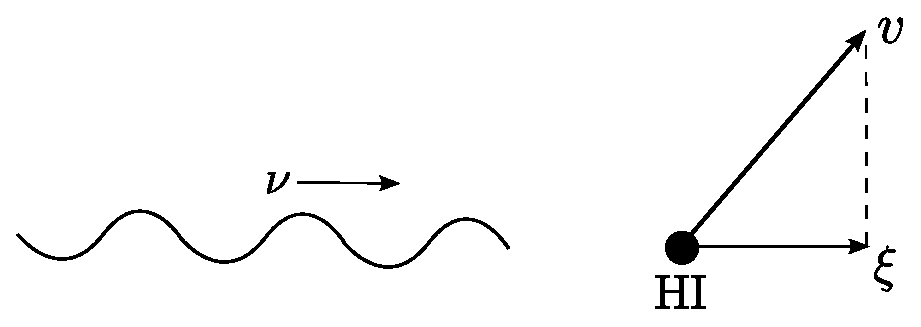
\includegraphics[width=8cm]{dopplerDiagram.eps}
  \caption{This diagram represents the process of Doppler broadening. The HI atom is moving away with velocity $v$ from incoming radiation with frequency $\nu$. The observed frequency of the radiation in the atom's rest frame is $\nu(1-\xi/c)$ where $\xi$ is the component of the velocity parallel with the incident radiation. }
  \label{fig:dopplerDiagram}
\end{figure}


where $T$ is the temperature of the gas, $\xi$ is the velocity and $k_{\text{B}}$ is the Boltzmann constant\gloss{$k_{\text{B}}$}{Boltzmann constant}Incident radiation will appear red/blueshifted in the frame of the absorbing atom with the shift being proportional to the atom's velocity \textit{parallel} to the incident radiation, as shown in Figure \ref{fig:dopplerDiagram}. Specifically, a photon with frequency $\nu$ will be observed by the atom to have frequency $\nu(1-\xi/c)$, where $\xi$ is the component of the atom's velocity \textit{away} from the incident radiation. Convolving our line profile with a Maxwell-Boltzmann distribution effectively involves replacing our expression in Eq. \ref{eq:IntroLineProfile} with

{\bf factors of $\lambda_{\alpha}??$}
\begin{align}
\sigma &\to \dfrac{\pi e^2}{m_e c}f_{\alpha}\lambda_{\alpha} \int_{-\infty}^{\infty} \dd \xi\ \phi(\nu(1-\xi/c)) W(\xi)\\
&= \dfrac{\pi e^2}{m_e c}f_{\alpha}\lambda_{\alpha} \int_{-\infty}^{\infty}\dd \xi\ \phi(\nu(1 - \xi/c)) \left(\pi \xi_{0}^{2} \right)^{-1/2} e^{-\xi^2/\xi_{0}^2} \\
&= \dfrac{\pi e^2}{m_e c} \frac{f_{\alpha}}{\pi} \left( \pi \xi_0^2 \right)^{-1/2} \int_{-\infty}^{\infty} \dd \xi \dfrac{(\Gamma/4\pi) e^{-\xi^2/\xi_{0}^{2}}}{(\nu-\nu_{0}(1-\xi/c))^2+(\Gamma/4\pi)^2}. \label{eq:IntroConvolution}
\end{align}

Here, we can make a couple substitutions and redefinitions:

\begin{align}
\Delta v_{\text{D}} &\equiv \nu_{0}\dfrac{\xi_{0}}{c} & y &\equiv -\xi/\xi_0 \\
v &\equiv \dfrac{\nu - \nu_{0}}{\Delta v_{\text{D}}} & a &\equiv \dfrac{\Gamma}{4\pi \Delta v_{\text{D}}}.
\end{align}

The quantity $\Delta v_{\text{D}}$ is known as the ``Doppler parameter" and is the red/blueshift in frequency space that the atom sees due to its thermal motion. The quantity $v$ is just the distance from line center in velocity space in units of the Doppler parameter. The quantity $a \equiv (\Gamma/4\pi)/\Delta v_{\text{D}}$ represents the ratio of the natural line width to the Doppler width. Rewriting our expression in Eq. \ref{eq:IntroConvolution}, we obtain

\begin{align}
\sigma(\nu) &= \dfrac{\pi e^2}{m_e c}f_{\alpha}\dfrac{1}{\sqrt{\pi}\Delta v_{\text{D}}} \dfrac{a}{\pi}\int_{-\infty}^{\infty}\dd y\ \dfrac{e^{-y^2}}{(v-y)^2+a^2}\\ 
&\equiv \dfrac{\sqrt{\pi} e^2}{m_e c} f_{\alpha}\dfrac{H(a,v)}{\Delta v_{\text{D}}}
\end{align}
where $H(a,v)$ is known as the Hjerting function \gloss{Hjerting Function}{Also known as the \textit{Voigt Function}, this function is commonly used in describing line profiles which incorporate Doppler broadening and the natural line width. This function is very relevant when studying the hydrogen damping wing.} or the Voigt function\gloss{Voigt Function}{Also known as the \textit{Hjerting Function}, this function is commonly used in describing line profiles which incorporate Doppler broadening and the natural line width. This function is very relevant when studying the hydrogen damping wing.}. So finally, we have obtained an expression for the \lya\ line profile incorporating the natural line width and Doppler broadening. Overall, the effect of the temperature acts to smear out the absorption line on scales of order $\sim 10\kms$ from line center. The greater the temperature, the larger the Doppler parameter and the greater the extent of the smearing. At scales $\gtrsim 100\kms$, the damping wing dominates the line profile. The profile is complex, but nonetheless, it encodes information about the underlying IGM temperature. Therefore, if simulations can generate accurate mock spectra for a variety of thermal histories, then comparisons between Voigt profile fits on the actual and mock spectra should be able to provide insight on the thermal properties of the IGM. 


This is the procedure undertaken by \cite{BoltonQuasar}. In Figure \ref{fig:QuasarProximityTemp}, they look for \lya\ absorption lines in the proximity zones of a high-redshift quasar in order to fit for the associated Doppler parameter and make inferences about the temperature. The top panel shows the fractional transmission for a mock quasar spectrum. The dashed curves indicate regions where absorption-line fitting was carried out and the vertical arrows indicate where the line centers were found from the fits. The second and third panel show the underlying temperature and density field, respectively. The bottom panel shows the true spectrum in question along with the same information regarding the line profile fits. These authors were able to use these fits to make inferences about the temperature of the IGM nearby the quasar. From these temperature measurements, and through comparison to mock spectra properties, these authors were able to place interesting limits on the ending of reionization ($z_{\text{H}} <  9$ assuming that the quasar reionizes its vicinity and Pop II stars drive reionization). This specific measurement is very difficult, however. The argument is essentially that the inferred temperature of the gas is too hot for reionization to have ended long before $z = 9$, otherwise the gas would have had more time to cool below the measured temperature. However, the regions nearby quasars should see a significantly-enhanced ionization field and all constraints made from measurements within this region hinge on ones ability to accurately account for such effects. 


The aforementioned technique for measuring the temperature is useful, but has the drawback that it requires a certain level of transmission in the quasar spectra in order to confidently fit a single absorption-line profile. However, at $z > 5$, individual absorption features blend together and the forest becomes somewhat inverted where, instead of stretches of transmission being punctuated with absorption features, stretches of absorption are punctuated with transmission features. This renders the goal of fitting for individual Voigt profiles impossible in the IGM. This also explains why \cite{BoltonQuasar} analyze the IGM  nearby a high-redshift quasar, where the transmission is enhanced due to the strengthened ionization field. 


An alternative approach to fitting line profiles is to measure the small scale power of the flux fluctuations (e.g., \citealt{Lidz2010}, \citealt{Theuns2002a}, \citealt{zaldarriaga2002searching}). This involves applying a localized wavelet filter to measurements of the \lya\ forest in order to measure the level of small-scale fluctuations. As we mentioned, large temperatures will lead to a larger Doppler parameter which will smear out small-scale structure. Thus, a large response to a small-scale wavelet filter would indicate significant small-scale structure and suggest a lower temperature for the gas. This approach has the important advantage that it doesn't rely on individual absorption lines to be discernible in order to extract temperature measurements. In \S \ref{sec:IGMTemperature}, we show that this can be used to constrain the IGM temperature at $z > 5$, \textit{even in typical regions of the IGM}.

%% Maybe we can defer discussion of this equation to chapter 3?
%\begin{align}
%\dfrac{\dd T}{\dd t} &= -2HT + \dfrac{2T}{3(1+\delta)}\dfrac{\dd \delta}{\dd t} + \dfrac{T}{\mu} \dfrac{\dd \mu}{\dd t} + \dfrac{2\mu m_p}{3\rho k_B}(\mathcal{H} - \Lambda) \label{eq:dtdt}
%\end{align}

\begin{figure}[h]
  \centering
  \includegraphics[width=11cm]{BoltonIGMTemperature_Fig2.ps}
  \includegraphics[width=11cm]{BoltonIGMTemperature_Fig2b.ps}
  \caption{This figure shows mock spectra, and corresponding simulated IGM properties, from \cite{BoltonQuasar} in the top four panels. The bottom panel shows the observed spectrum from SDSS J0818+1722, which \cite{BoltonQuasar} use in order to make temperature measurements inside the proximity zone. Dashed lines indicate regions where Voigt-profile fitting was performed and downward arrows indicate the detected centers of the Voigt profiles. {\bf Maybe Bolton and Becker is better to use here? Larger sample of quasars, same basic idea...}}
  \label{fig:QuasarProximityTemp}
\end{figure}


\subsubsection{Motivation for this Work}

This discussion of the \lya\ forest as a tool for constraining the EoR highlights several of the current drawbacks of the approach. Among these, the largest is arguably the degeneracy between different sources of saturated absorption in the \lya\ forest. If one could find a way to determine if absorption in the \lya\ forest was certainly happening as a result of underlying neutral hydrogen, then it would be easier to interpret observations in terms of the overall neutral fraction of the Universe. We highlighted one example of how this has been done: the hydrogen damping wing redward of \lya. While a useful approach, this also suffers from drawbacks of its own, namely the limited number of high-redshift spectra suitable for damping-wing searches and the fact that regions surrounding quasars are not expected to be representative of the IGM as a whole. This helps motivate two approaches we consider in \S \ref{sec:NeutralIslands}. Namely, we identify the hydrogen damping wing and absorption due to deuterium as ``smoking gun" signals of underlying hydrogen and search for them in typical regions of the IGM. Obviously, it will become clear that this approach suffers from its own drawbacks but it does provide an independent measurement useful for constraining the ionization state of the high-redshift IGM.

Second, we have discussed some difficulty in making measurements of the temperature of the high-redshift IGM. Namely, due to the high levels of absorption in the \lya\ forest of quasar spectra at these redshifts, traditional methods of inferring the IGM temperature are inapplicable except in the highly-complex near-zones of quasars. This motivates the development of a temperature-measurement technique which is applicable to typical regions of the high-redshift IGM. Such a technique is proposed in {\bf cite} and discussed in \S \ref{sec:IGMTemperature}.

\subsection{The 21-cm Line}

The 21-cm line refers to the hyperfine splitting of the hydrogen atom where, due to the interaction between the magnetic dipole moments\gloss{Magnetic Dipole Moment}{The magnetic dipole moment of an object is related to the torque it would experience when placed in an external magnetic field. Magnetic moments are often relevant for bar magnets or loops of current. In the context of the hydrogen atom, the spin of the proton and electric render them as a sort of ``loop of current'' which gives them their own magnetic dipole moment.} of the electron and proton in, a small energy difference exists between the configuration where the spins of the electron and proton are aligned versus where they are anti-aligned. The configuration where the spins are anti-aligned (and magnetic dipole moments are therefore aligned) is energetically favored and has a lower energy by $\Delta E \approx 6\times 10^{-6}$eV.\footnote{This is in contrast to a \lya\ photon which has energy $E \approx 10.2\text{eV}$, more than a million times greater.} Thus, spin-flip transitions will result in (from) the emission (absorption) of a photon with $\lambda \approx 21\cm$, $\nu \approx 1420\mhz$. This is shown schematically in Figure \ref{fig:21cmline}. 


As we discussed in \S \ref{sec:LyaForest}, the cross section or the \lya\ transition is extremely large, which presents us with a host of difficulties. However, the 21-cm transition is a ``forbidden'' transition\gloss{Forbidden Transition}{This refers to atomic transitions which are not allowed under the quantum mechanical selection rules under the dipole approximation. Essentially, this means the transitions are relatively extremely rare compared to ``allowed'' transitions.}, meaning its rate of occurrence is extremely low. As a result, the Universe is essentially transparent to 21-cm photons, allowing them to travel unimpeded from distant neutral hydrogen to us. In principal, this allows us to observe the hydrogen density field directly up to redshifts of $z \gtrsim 50$, \textit{far beyond the timescale of reionization} and far beyond the reach of the \lya\ forest. Measurements of the evolution of the 21-cm signal with redshift would allow us to construct something like a reionization ``movie'', which would constitute the ultimate constraint on reionization. 


Mapping the intensity of the 21-cm line during reionization avoids many other drawbacks of the \lya\ line as well. Namely, intensity mapping would provide us with a 3D volume of intensity values, as opposed to the \lya\ forest which is typically observed one sightline at a time. Also, since we are directly observing the hydrogen, we are not forced to make controversial assumptions about the state of the gas in order to interpret the results. 

In this section, let us start with a overview of the physics of the 21-cm line and then continue by discussing a couple avenues by which the 21-cm signal could be utilized in order to constrain reionization. 


\subsubsection{The Intensity of the 21-cm Line}\label{sec:21cmPhysics}


We mentioned above that hydrogen gas will ``dimly glow'' with 21-cm radiation, but exactly how dim? Let us start by considering the brightness of a distant hydrogen gas cloud.\footnote{This discussion will closely follow \S 2.1 of \citealt{Furlanetto2006}, which is an excellent review of the 21-cm line.} This is usually described in terms of a \textit{specific intensity} and then in terms of a \textit{brightness temperature}\gloss{Brightness Temperature ($T_b(\nu)$)}{An object with a given specific intensity $I_{\nu}$ has a corresponding brightness temperature equal to the requisite temperature of a blackbody for its specific intensity to equal that of the object, $I_{\nu} = B_{\nu}(T_{b}(\nu))$.}\gloss{Specific Intensity ($I_{\nu}$)}{The specific intensity of light leaving a cloud of gas is the energy carried by the light per unit frequency, area, time, and solid angle.}. The specific intensity of light leaving our HI cloud is the amount of energy per unit frequency, time, area, and solid angle, denoted $I_{\nu}$. The brightness temperature is the required temperature of a blackbody to radiate with the same specific intensity at that frequency, i.e., $B_{\nu}(T_b) = I_{\nu}$, where $B_{\nu}$ denotes the blackbody spectrum. 


The light we observe from our HI cloud will be a combination of background light shining \textit{through} the cloud and light emitted by the cloud itself. This follows the radiative transfer equation (in the clouds frame)

\begin{align}
T_b(\nu) &= T_{\text{cloud}}(1-e^{-\tau_{\nu}}) + T_{\text{background}}e^{-\tau_{\nu}} \label{eq:cloudframe}
\end{align}
where the background light is from the CMB, such that $T_{\text{background}} = 2.73\text{K}(1+z)$, and $T_{\text{cloud}}$ is the \textit{spin temperature}, defined below. The quantity $\tau_{\nu}$ is the frequency-dependent optical depth for absorption \textit{by} the HI cloud. This is equal to 

\begin{align}
\tau_{\nu} &= \int \dd s \sigma_{01}\left( 1 - e^{-E_{10}/k_{\text{B}}T_{\text{S}}} \right) \phi(\nu) n_{0} \label{eq:tau21}
\end{align}

where the integral is carried out along the line of sight through the cloud. In this expression, $E_{10} \approx 6\times 10^{-6}$eV is the energy of the transition, $\phi(\nu)$ is the line profile, $\sigma_{01}$ is the cross-section for 21-cm absorption by a hydrogen atom and $n_{0}$ is the number density of hydrogen atoms in the unexcited state. We follow the convention of \cite{Furlanetto2006} and denote the lower energy level by ``0'' and the higher energy level by ``1''. The ratio of the population of atoms in the excited state to the ground state is defined by the spin temperature and the degeneracy of the states:

\begin{align}
\dfrac{n_{1}}{n_{0}} &= \dfrac{g_1}{g_0}e^{-E_{10}/k_{\text{B}}T_{\text{S}}} = 3 e^{-E_{10}/k_{\text{B}}T_{\text{S}}}.
\end{align}

The excited state is the triplet state and has a three-fold degeneracy: $|\uparrow \uparrow \rangle$, $\dfrac{1}{\sqrt{2}}(|\uparrow \downarrow\rangle + |\downarrow \uparrow \rangle)$, $|\downarrow \downarrow\rangle$, and the lower-energy state is the singlet state: $\dfrac{1}{\sqrt{2}}( |\uparrow \downarrow\rangle - |\downarrow \uparrow \rangle)$. $T_{\text{S}}$ is the spin temperature and is defined via this equation. For our purposes, $T_{\text{S}} \gg E_{10}/k_{\text{B}}$, so we have $n_{1}/n_{0} = 3$ and

\begin{align}
1 - e^{-E_{10}/k_{\text{B}}T_{\text{S}}} &\approx \dfrac{E_{10}}{k_{\text{B}}T_{\text{S}}}
\end{align}


 Furthermore, since only one out of four hydrogen atoms are in the singlet state, $N_{\text{HI}}/4 = \int \dd s n_{0}$. Putting this together, Eq. \ref{eq:tau21} becomes
 
\begin{align}
\tau_{\nu} &\approx \sigma_{01} \dfrac{N_{\text{HI}}}{4} \dfrac{E_{\text{10}}}{k_{\text{B}}T_{\text{S}}} \phi(\nu)
\end{align}
where 
\begin{align}
\sigma_{01} &\equiv \dfrac{3c^2 A_{10}}{8\pi\nu^{2}}
\end{align}

where $A_{10} = 2.85 \times 10^{-15}\sec^{-1}$ is the spontaneous emission coefficient for the transition. As we discussed in \S \ref{sec:IntroIGMTemperature}, line profiles depend on several properties of the gas, however, here it is the case that Doppler broadening due to the expansion of the Universe dominates the line profile, such that

\begin{align}
\phi(\nu) \approx \dfrac{c}{s H(z) \nu}.
\end{align}

Putting these pieces together, our expression for the optical depth becomes:

\begin{align}
\tau_{\nu} &\approx \dfrac{3c^2 A_{10}}{8\pi \nu^{2}} \dfrac{h \nu}{k_{\text{B}}T_{\text{S}}} \dfrac{c}{s H(z) \nu} \dfrac{n_{\text{HI}}\langle x_{\text{HI}}\rangle s}{4} \tag{$N_{\text{HI}} = s n_{\text{HI}}\axhi$}\\
&\approx \dfrac{3hc^3 A_{10}}{32\pi \nu^2 k_{\text{B}}T_{\text{S}}} \dfrac{n_{\text{HI}}\axhi}{H(z)}
\end{align}
plugging in values and evaluating at line center, \cite{Furlanetto2006} obtain

\begin{align}
\tau_{\nu_{0}} &\approx 0.0092 (1+\delta)(1+z)^{3/2}\dfrac{\axhi}{T_{\text{S}}}\left[ \dfrac{H(z)/(1+z)}{\dd v_{\parallel}/\dd r_{\parallel}} \right] 
\end{align}

where $\dd v_{\parallel}/\dd r_{\parallel}$ is the gradient in the line-of-sight velocity (peculiar velocity and velocity due to Hubble expansion) and the ratio of that with $H(z)/(1+z)$ represents the deviation from pure-Hubble expansion. For the purposes of the 21-cm probes we will discuss, we actually care about the \textit{contrast} between the 21-cm signal and the background CMB signal. Thus, the relevant brightness temperature contrast, in our frame, is 

\begin{align}
\delta T_{b} &= \dfrac{1}{1+z}\left[ T_{\text{S}}(1-e^{-\tau_{\nu_{0}}}) + T_{\text{CMB}}e^{-\tau_{\nu_{0}}} - T_{\text{CMB}} \right] \\
&= \dfrac{T_{\text{S}}-T_{\text{CMB}}}{1+z} (1 - e^{-\tau_{\nu_{0}}}) \\
&\approx \dfrac{T_{\text{S}}-T_{\text{CMB}}}{1+z} \tau_{\nu_{0}} \\ 
&\approx 9\text{mK}\cdot x_{\text{HI}}(1+\delta)(1+z)^{1/2}\left[ 1 - \dfrac{T_{\text{CMB}}}{T_{\text{S}}} \right] \left[ \dfrac{H(z)/(1+z)}{\dd v_{\parallel}/ \dd r_{\parallel}} \right] \\ 
&\approx 24 \text{mK}\cdot x_{\text{HI}}(1+\delta)\left(\frac{1+z}{7}\right)^{1/2}\left[ 1 - \dfrac{T_{\text{CMB}}}{T_{\text{S}}} \right] \left[ \dfrac{H(z)/(1+z)}{\dd v_{\parallel}/ \dd r_{\parallel}} \right].
\end{align}

Thus, we see that a neutral parcel of hydrogen at mean density and $z = 6$ and $T_{\text{S}} \gg T_{\text{CMB}}$, the brightness temperature contrast is $\sim 24\text{mK}$.




\begin{figure}[h]
  \centering
  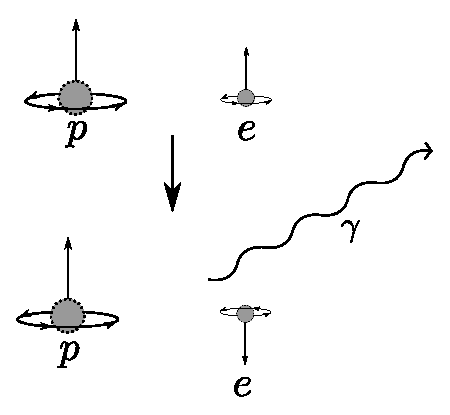
\includegraphics[width=8cm]{21cmline.eps}
  \caption{Schematic representation of the 21-cm transition where the transition between aligned spins of the proton and electron to anti-aligned spins results in the emission of a photon with $\lambda \approx 21$cm. }
  \label{fig:21cmline}
\end{figure}

\begin{figure}[h]
  \centering
  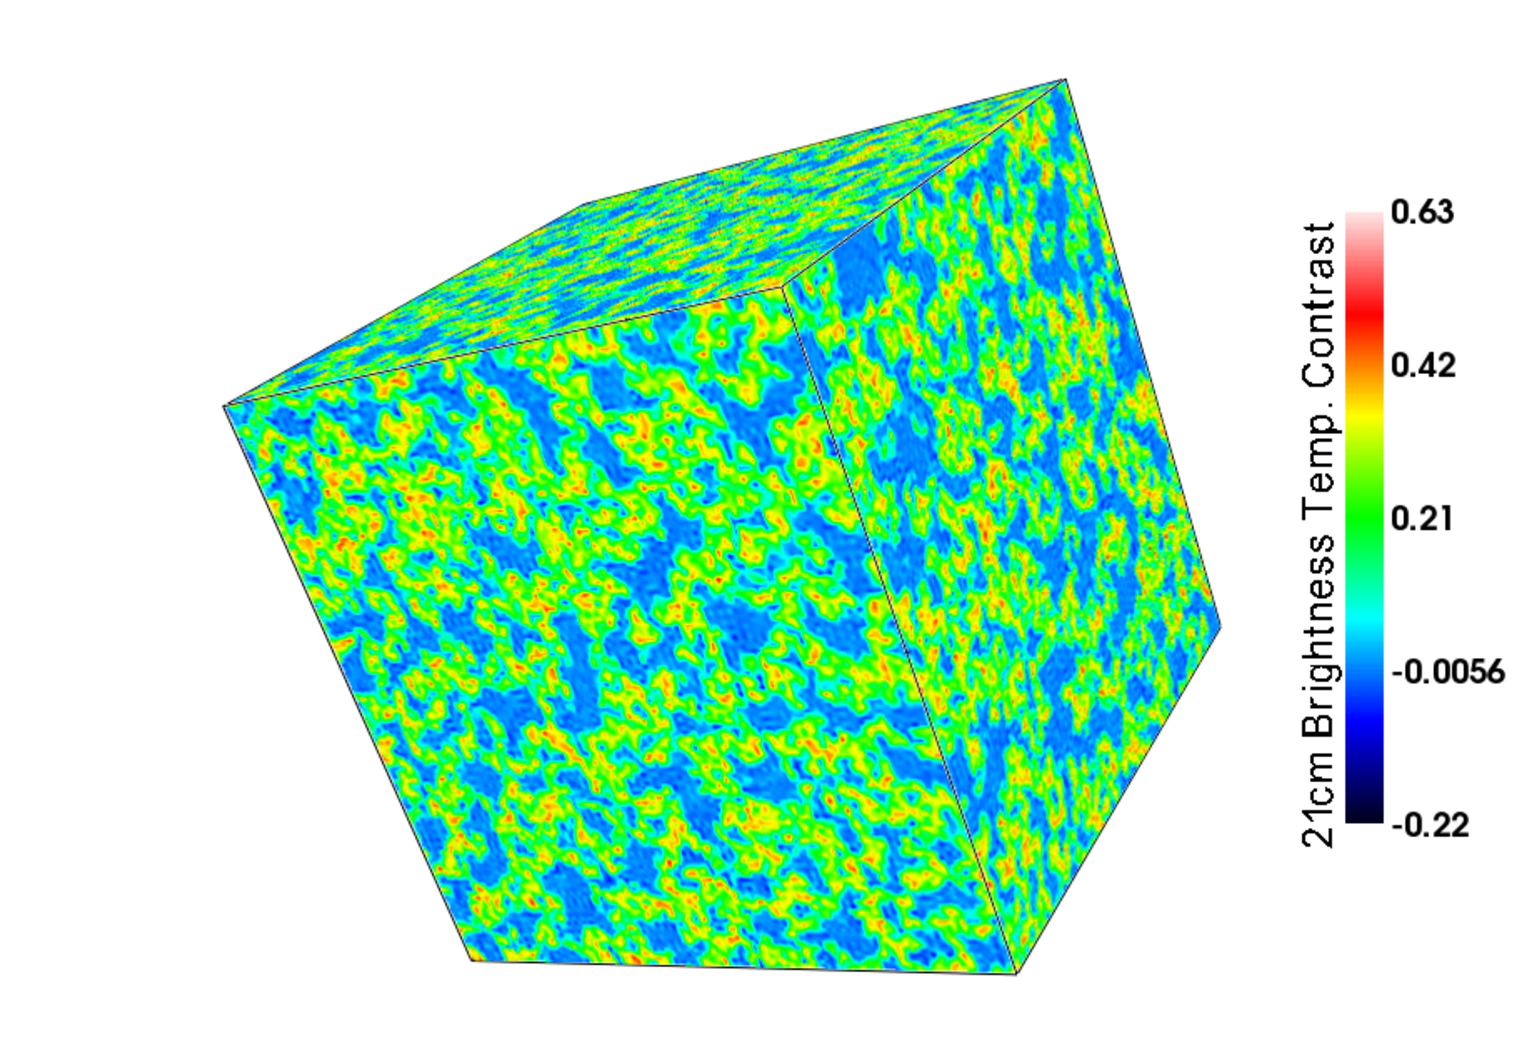
\includegraphics[width=8cm]{TalkSignal.eps}
  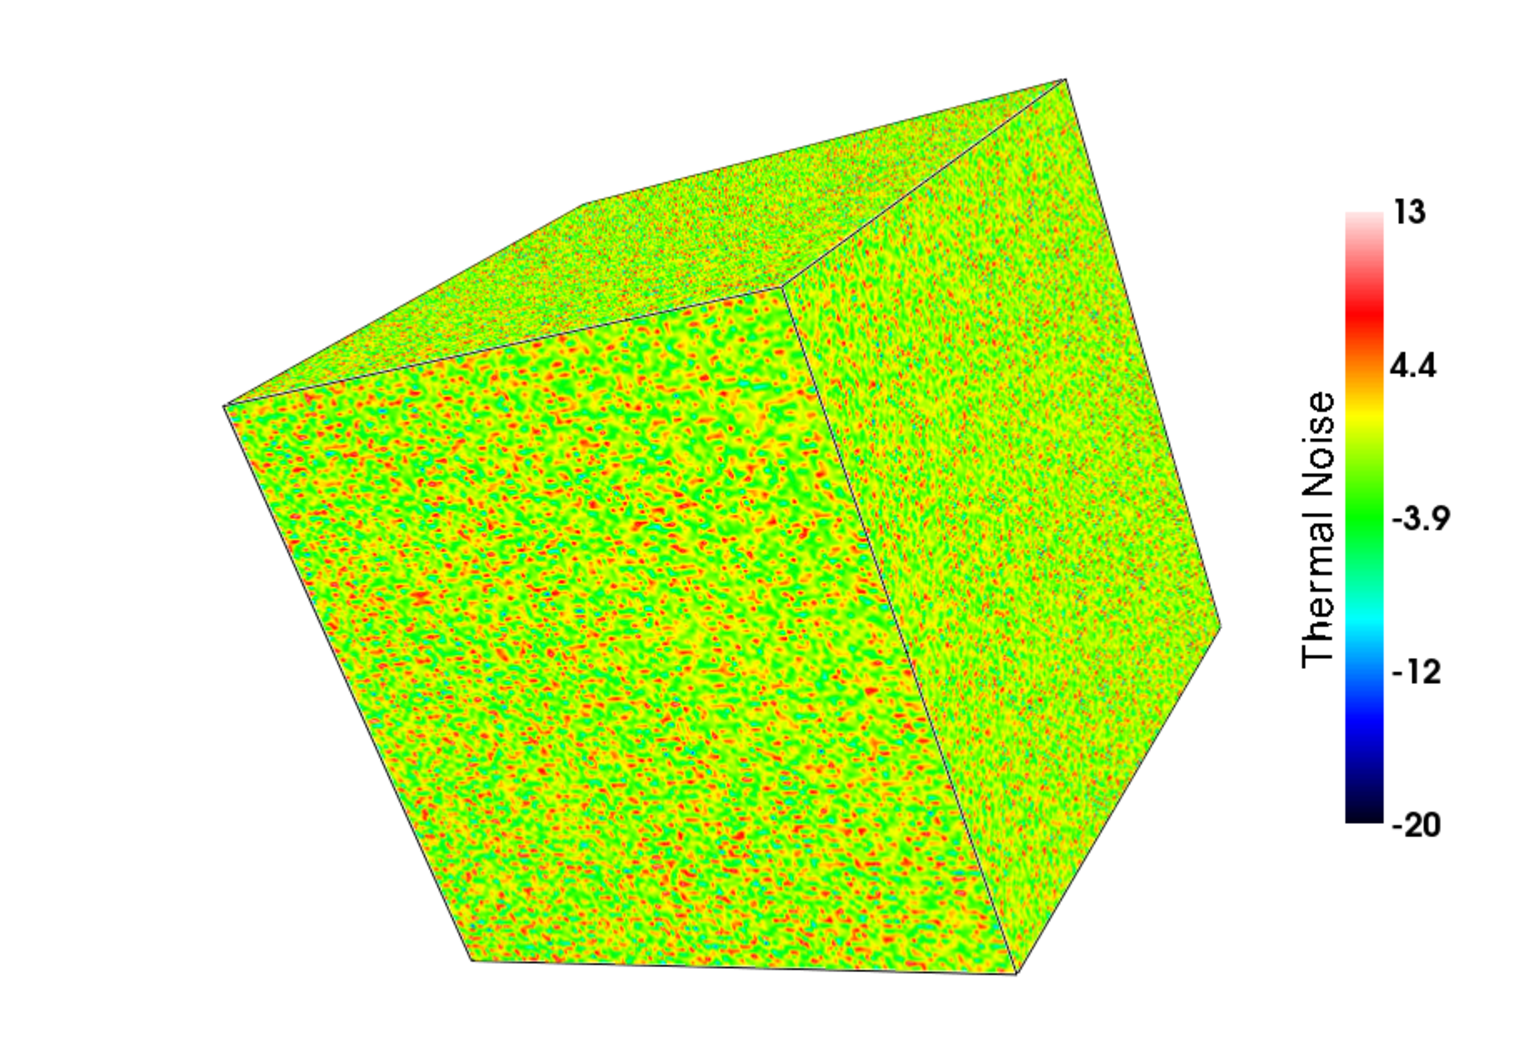
\includegraphics[width=8cm]{TalkNoise.eps}
  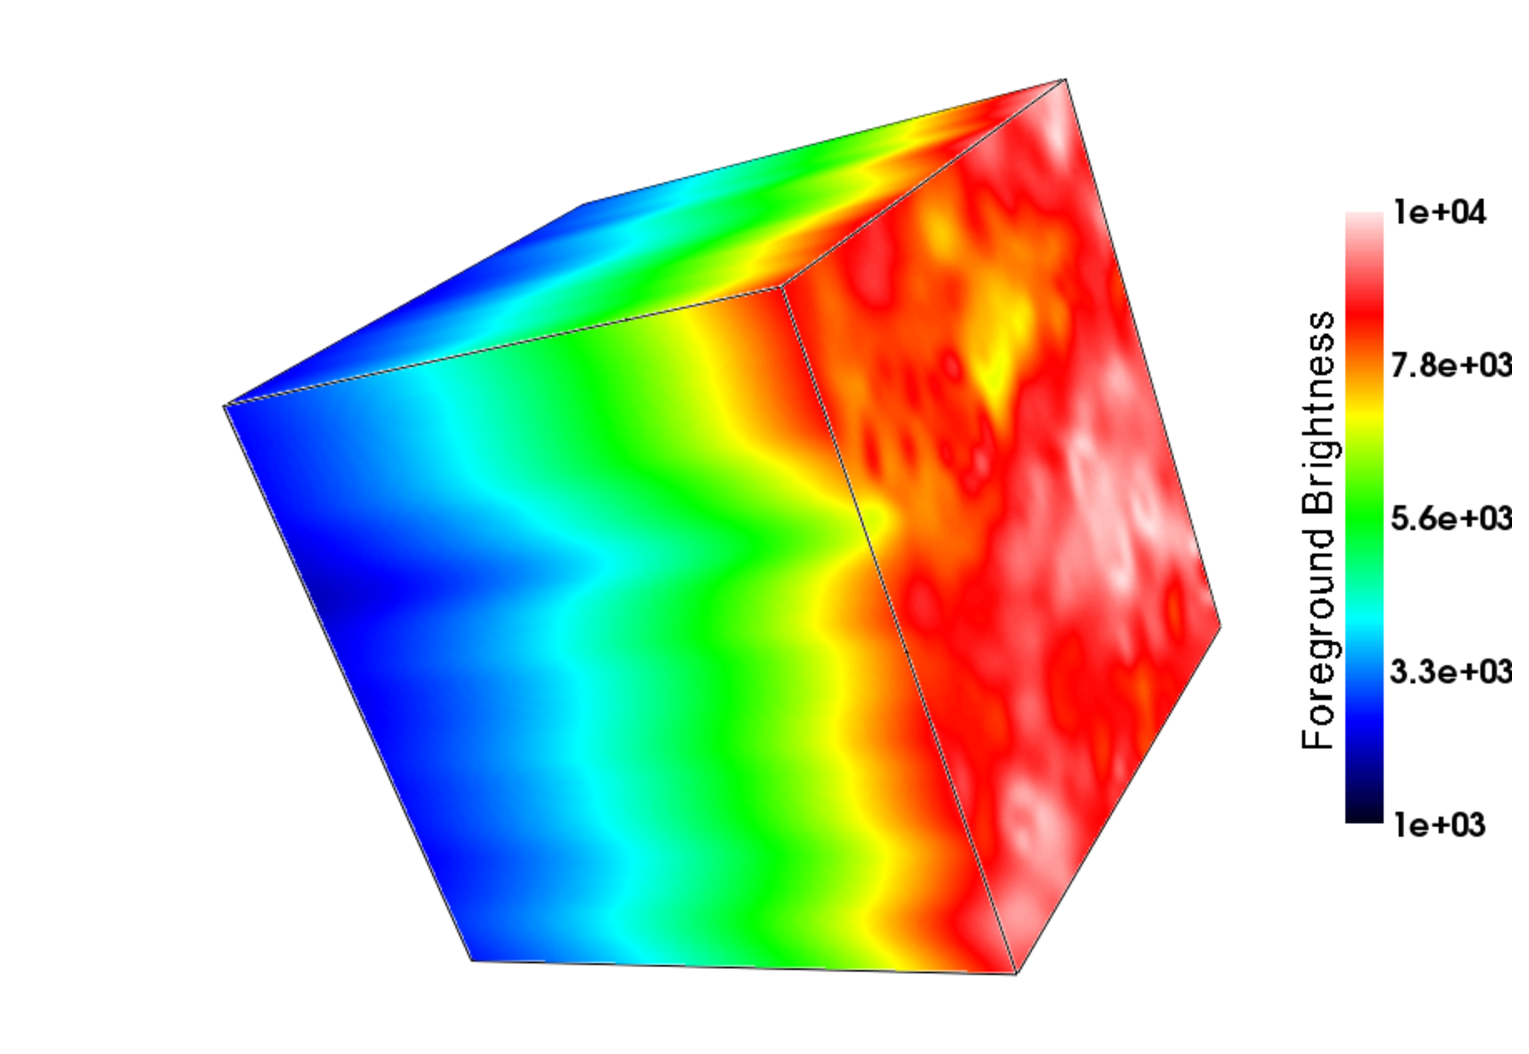
\includegraphics[width=8cm]{TalkFG.eps}
  \caption{Simulation cube of the 21-cm signal during reionization (top) along with simulated noise for an interferometer (middle) and the galactic foregrounds (bottom). This figure demonstrates that, while the sources of noise are several orders of magnitude larger than the signal, these three contributions to observations are dominant of different scales. The volume of each cube is 1 $(\text{Gpc}/h)^{3}$. In this figure, the line of sight direction away from the observer is to the right. }
  \label{fig:21cmCube}
\end{figure}

\subsubsection{The Global 21-cm Signal}

An alternative method of extracting information from the 21-cm line is to use the \textit{sky-averaged} 21-cm signal. In the previous section, we discussed the difficulties faced in obtaining the necessary resolution to map out fluctuations in the 21-cm radiation field. However, Equation \ref{eq:dTb} is rich with astrophysical information on its own without even considering spatial fluctuations. Therefore, natural questions to ask would be if it is easier to simply measure the average signal rather than map the fluctuations and what astrophysical information can be obtained in that way? For convenience, the brightness temperature contrast for the 21-cm signal from \S \ref{sec:21cmPhysics} is:

\begin{align}
\delta T_{b} &\approx 24 \text{mK}\cdot x_{\text{HI}}(1+\delta)\left(\frac{1+z}{7}\right)^{1/2}\left[ 1 - \dfrac{T_{\text{CMB}}}{T_{\text{S}}} \right] \left[ \dfrac{H(z)/(1+z)}{\dd v_{\parallel}/ \dd r_{\parallel}} \right].
\end{align}

As mentioned earlier, for the end of reionization, the dependence on the spin temperature drops out. The result is that the amplitude of a sky-averaged signal  would be most sensitive to the neutral faction, with ionized regions emitting no 21-cm signal. Thus, one could imagine plotting the sky-averaged 21-cm signal against redshift and observing a shrinking signal coinciding with the EoR. 


However, the utility of the global 21-cm signal is not limited to the Epoch of Reionization. Specifically, prior to reionization, $\axhi$ will be fixed at 1 and the spin temperature is expected to drop to the point where $1 - T_{\text{CMB}}/T_{\text{S}} \not\approx 1$. This is interesting because the spin temperature itself depends on several astrophysical processes. A very high-level description of this is shown in Figure \ref{fig:TsEvolution}.\footnote{This figure and much of the following discussion is taken from notes from Adam Lidz's ``Topics in Cosmology'' class, taught in the Fall of 2011.} The precise evolution of the spin temperature is not well known, but a reasonable approximate description could be as follows:

\begin{enumerate}
\item [] \underline{$z > 150$:} Collisions within the gas are frequent enough to fix the spin temperature to the gas temperature, $T_{\text{S}} = T_{\text{K}}$. However, the gas temperature is equal to the CMB temperature, so the 21-cm signal is \textit{unobservable}.
\item [] \underline{$30 < z < 150$:} Collisions are efficient at coupling the gas temperature to the spin temperature. Furthermore, the gas cools to below the CMB temperature, making the 21-cm signal \textit{obervable}. 
\item [] \underline{$20 < z < 30$:} The gas density drops enough so that collisions are not efficient at coupling the spin temperature to the gas temperature. As a result, the spin temperature approaches the CMB temperature and the 21-cm signal is \textit{unobservable}. 
\item [] \underline{$15 < z < 20:$} Wouthuysen field effect re-couples the spin temperature to the gas temperature, which is still below the CMB temperature. This renders the 21-cm signal \textit{observable in absorption}. 
\item [] \underline{$ z < 15:$} The first X-ray sources form and heat the gas well above the CMB temperature. As a result, the 21-cm signal becomes \textit{observable in emission}.
\item [] \underline{$ z \lesssim 5.5:$} The completion of reionization effectively eliminates the 21-cm signal from the IGM all together. The 21-cm signal is still observable in pockets of neutral gas surrounding galaxies. 
\end{enumerate}


\begin{figure}[h]
  \centering
  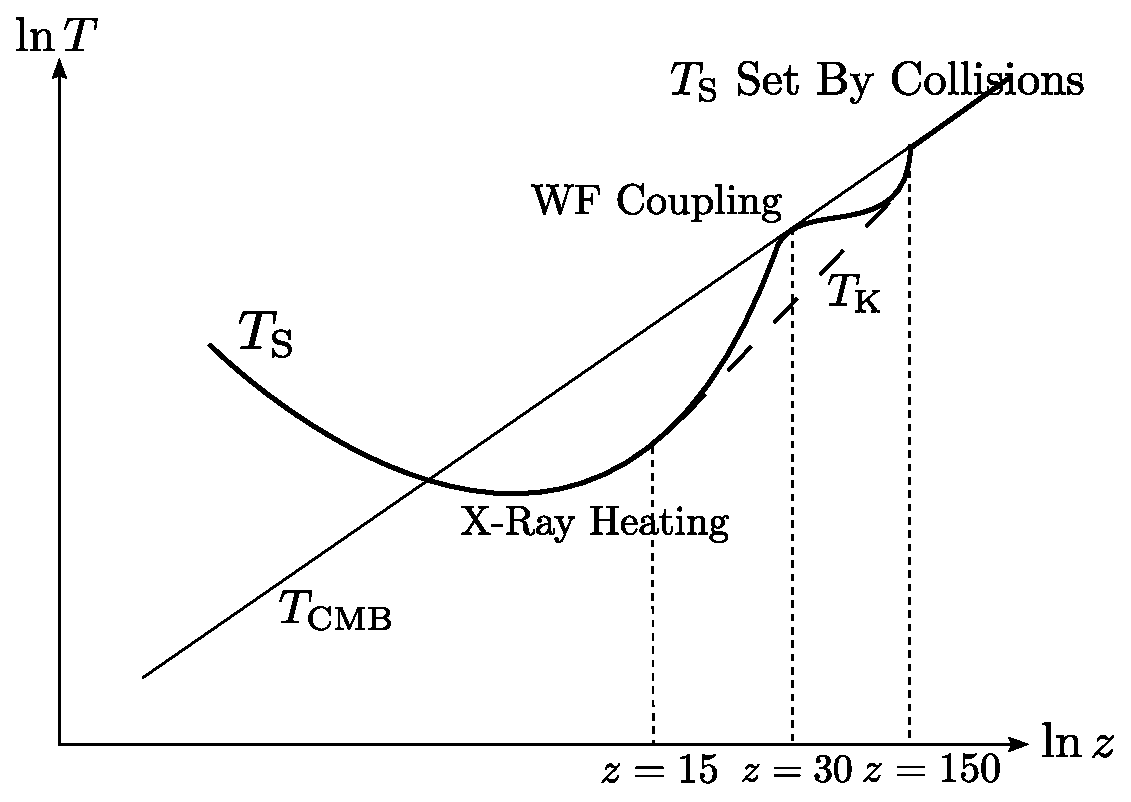
\includegraphics[width=12cm]{TsEvolution.eps}
  \caption{Schematic representation of a plausible $T_{\text{S}}$ signal including a few landmarks. This is adapted from notes taken in the course ``Topics in Cosmology''.}
  \label{fig:TsEvolution}
\end{figure}



\subsection{The Cosmic Microwave Background}\label{sec:CMB}
\subsection{\lya\ Emitters}

\lya\ emitters (LAEs)\gloss{LAE}{\lya\ Emitter. These are galaxies which emit a significant fraction of their energy in the \lya\ line. This line is produced when hydrogen atoms within the galaxy recombine after being ionized by the galaxy. Roughly 2/3 of recombinations result in a \lya\ photon.} are galaxies which emit strongly in the \lya\ line. This \lya\ emission results from hydrogen atoms within the galaxy recombining after being ionized by the galaxy's UV radiation. During $\sim2/3$ of hydrogen recombinations, a \lya\ photon will be emitted. Therefore,  enough ionizations will result in a strong \lya\ line being emitted from the galaxy. 


However, whether or not that \lya\ line is observable to us depends on the intervening gas. Specifically, \lya\ photons produced within the galaxy will repeatedly be absorbed and re-emitted by hydrogen in the galaxy's interstellar medium until it reaches the IGM. At this point, if the IGM is ionized the \lya\ photon will escape. However, if the IGM is significantly neutral, then the \lya\ photon will be scattered into a low-surface-brightness halo, rendering the \lya\ line unobservable (\citealt{finlator2012recent}). This provides us with an observable which depends on the ionization state of the IGM! In this section, we briefly discuss two methods of utilizing this behavior in order to constrain $\axhi$.

%at \axhi = 0.5, LAEs residing in HII regions will typically be one of thousands that contribution to ionizing the HII regions. These regions can be \sim 10 Mpc. However, lya photons only need to travel 1 Mpc in order to redshift out of resonance and escape. 

\subsubsection{Clustering of \lya\ Emitters}

One approach for utilizing LAEs to constrain $\axhi$ is to look at their measured clustering. When the IGM is fully-ionized, the \lya\ lines of all observed galaxies should be visible to us. When the Universe is fully-neutral, then all observed galaxies should lack a strong \lya\ emission line. However, when reionization has progressed such that $\axhi \approx 0.5$, the Universe should represent a two-phase medium consisting of large ($\sim 10\mpch$) ionized regions maintained by thousands of galaxies (\citealt{McQuinn:2007dy}), and significantly-neutral regions which are shielded from the ionizing radiation. The \lya\ line from LAEs located within the large ionized regions should remain intact, as the photons will redshift out of \lya\ resonance after travelling only $\sim 1\mpch$ without encountering significantly-neutral hydrogen (\citealt{finlator2012recent}). Therefore, the LAEs observable when the Universe is 50\% ionized should more often reside in these ionized bubbles with many other sources, resulting in their observed distribution being \textit{highly clustered}. Meanwhile, at lower redshift, all LAEs should be observable (with regard to HI attenuation), resulting in a more uniform distribution.

In Figure \ref{fig:McQuinnLAEClustering}, \cite{McQuinn:2007dy} demonstrate this effect. The top row shows the ionization field (black is neutral, white is ionized) at three different neutral fractions: $\axhi = 0.7$ (left), 0.5 (middle), and 0.3 (right). The second row shows the true underlying LAE locations and the bottom row shows the observed LAEs. Since LAEs should only be observable within ionized regions, we see that the sources in the bottom row must coincide with white regions in the top row, resulting in enhanced clustering of the observed sources.

In \cite{Ouchi2010}, the authors analyze 207 LAEs at $z \sim 6-7$ and compare their clustering with those measured at $z = 5.7$. They find no detection of an enhancement in the observed LAE clustering, suggesting that the bulk of reionization occurred at $z > 6.6$. 



\begin{figure}[h]
  \centering
  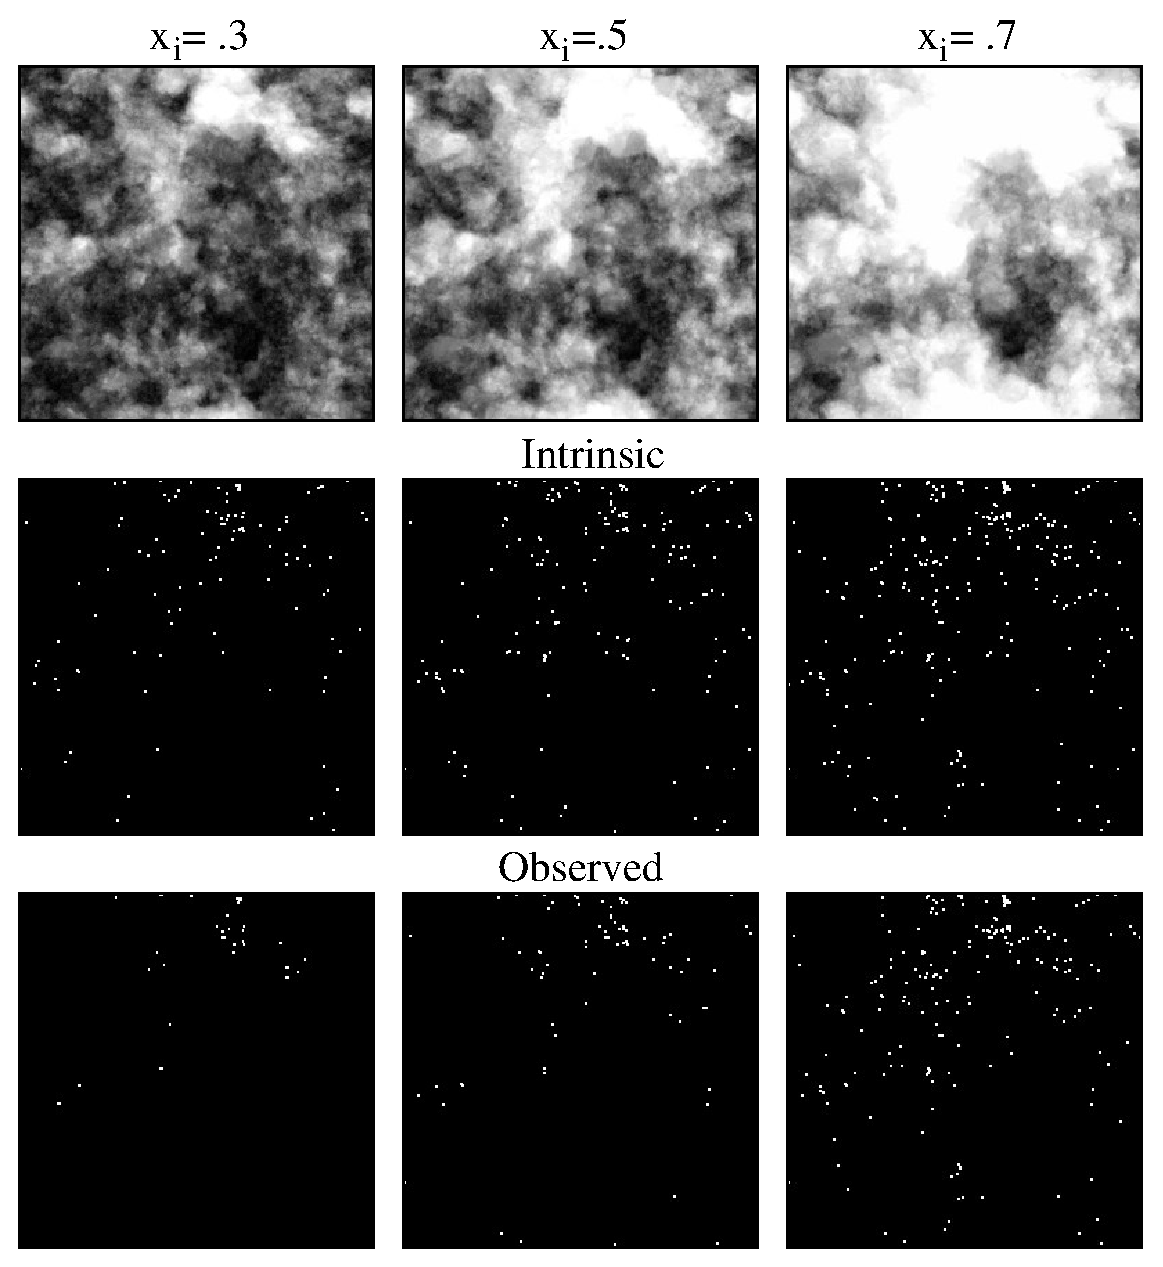
\includegraphics[width=13cm]{McQuinnLAEClusteringLarge.eps}
  \caption{The effect of the neutral fraction on the observed clustering of LAEs (taken from \citealt{McQuinn:2007dy}). The top panels show the underlying ionization fields, the middle row shows the true location of LAEs in the simulation, and the bottom panel shows the detectable LAEs in the simulation. This shows that, LAEs which occupy the same ionized bubble will be observable, resulting in a less homogeneous field of observable LAEs. Each panel is 94 Mpc across. }
  \label{fig:McQuinnLAEClustering}
\end{figure}


\subsubsection{\lya\ Emitter Fraction}

As discussed in the previous section, as we move further back in redshift and deep into the reionization process, galaxies that intrinsically have a significant \lya\ line will not be observed as having one. However, the galaxies themselves will still be detectable via the drop-out technique, which searches for sources with significant emission at energies below the Lyman limit\gloss{Lyman Limit}{This refers to the most energetic transition in the Lyman series corresponding to ionizing a hydrogen atom in the ground state. This has wavelength $\lambda = 912$\AA and $E_{\gamma} = 13.6$eV.} and significantly less emission at greater energies. 


As we move further back in redshift, we expect the fraction of detected galaxies which \textit{would} have a \lya\ line but do not, due to a significantly-neutral IGM, will increase. While we do not have access to this exact measurement of this fraction, we \textit{can} measure the \textit{overall} fraction of detected galaxies which exhibit a strong \lya\ line, which should reflect the aforementioned trend. This has motivated the study of the evolution of the so-called ``\lya\ fraction'', denoted $f_{\text{\lya}}$ (\citealt{Schenker2012,pentericci2011spectroscopic,Pentericci:2014nia,caruana2012no,caruana2014spectroscopy}). This method has the benefit compared to some others, such as measuring the LAE luminosity function evolution, that some uncertainties due to the overall redshift evolution of observable galaxies, unrelated to the EoR, will drop out. 


Interestingly enough, some of these authors' analyses claim to support a surprisingly-neutral IGM. Specifically, work by \cite{caruana2014spectroscopy}, \cite{Pentericci:2014nia}, \cite{pentericci2011spectroscopic}, and \cite{Schenker2012} all suggest a neutral fraction of $\langle x_{\text{HI}}(z \sim 7) \rangle \sim 0.5$. This seems to be in tension with other constraints on the reionization process. Namely, in \S \ref{sec:CMB}, we discussed constraints on the redshift of ``instantaneous reionization'', which can be interpreted as an upper bound on the mid-point of reionization, of $z_{r} = 8.8^{+1.3}_{-1.2}$ (\cite{planck2015planck}). Additionally, analysis by \cite{Bolton:2007b} suggests that reionization is a rather extended process. Assuming this $f_{\text{Ly}\alpha}$ constraint is correct, this would allow only $\Delta z \sim 1$ for the second half of reionization to complete. 


One plausible way to reconcile these observations is presented by \cite{2013MNRAS.429.1695B} who suggest that the rise in the prevalence of dense absorbers at high $z$, rather than a rise in the neutral fraction of the diffuse IGM, could contribute to a surprisingly-small $f_{\text{Ly}\alpha}$ without requiring changes in the neutral fraction of tens of per cent over $z \sim 6-7$. Furthermore, \cite{Taylor:2013qia} argue that, due to the expected large-scale inhomogeneity of reionization, LAE surveys which sample relatively small regions of the sky are subject to sample variance which can mitigate the high-neutral-fraction requirements. However, their analysis still suggests that $\axhi > 0.05$ at 95\% confidence. Thus, while the precise amount of neutral hydrogen required to explain the $f_{\text{Ly}\alpha}$ observations is controversial, it is exciting that the conclusion we are observing some phase of reionization is rather robust. 

% papers to cite
% detect something
% \cite{Schenker2012}
% \cite{pentericci2011spectroscopic}
% \cite{Pentericci:2014nia}
% \cite{Pentericci:2014nia}
% \cite{caruana2012no}
% \cite{caruana2014spectroscopy}
% don't
% 


\subsection{Luminosity Function Measurements}

\section{Where We Stand}

%\begin{enumerate}
%\item Bouwens et al. (2015) might be good to include here. Strengthens argument that galaxies reionized the Universe and that quasars/AGN did not.
%\end{enumerate}
% ----------------------------------------------------------------------



